%%%%%%%%%%%%%%%%%%%%%%%%%%%%%%%%%%%%%%%%%%%%%%%%%%%%%
%% File: main.tex
%% Author: John Liaperdos (ioannis.liaperdos@gmail.com)
%%Edited by: Jordi Jaromil Cruz- %%Medrano(jordi.cruz@uppuebla.edu.mx)
%%%%%%%%%%%%%%%%%%%%%%%%%%%%%%%%%%%%%%%%%%%%%%%%%%%%%
\documentclass[modern,hyperref,histinit,frontispiece]{teipel-thesis-en}
\usepackage{xcolor}
\usepackage{graphicx}
\definecolor{uppue}{HTML}{330033}
\graphicspath{{figures/}}
\usepackage{appendix}

%%%%%%%%%%%%%%%%%%%%%%%%%%%%%%%%%%%%%%%%%%%%%%%%% QUITE EL % A  LA ESPECIALIDAD QUE PERTENEZCA, LOS OTROS DEBERÁN DE TENER EL %  
%%%%%%%%%%%%%%%%%%%%%%%%%%%%%%%%%%%%%%%%%%%%%%%%%
	\DepartmentName{Maestría en Ingenería en Sistemas y Cómputo Inteligente}
	%\DepartmentName{Maestría en Ingeniería en Automatización de Procesos Industriales}
    	%\DepartmentName{Maestría en Ingeniería en Diseño de Bioprocesos}
        	%\DepartmentName{Maestría en Gestión e Innovación Tecnológica}
            	%\DepartmentName{Maestría en Enseñanza de las Ciencias}
                %\DepartmentName{Maestría en Gestión e Innovación Tecnológica}
%\DepartmentName{Maestría en Enseñanza de las Ciencias}
%%%%%%%%%%%%%%%%%%%%%%%%%%%%%%%%%%%%%%%%%%%%%%%%% CAMBIAR POR TUS DATOS 
%%%%%%%%%%%%%%%%%%%%%%%%%%%%%%%%%%%%%%%%%%%%%%%%%

% Titulo de la tesis  
	\title{Servicio web para la extracción de información semántica del RI-UPPue}
% Nombre de quien realizo la tesis 
	\authorName{Ing. Paulo Daniel Vázquez Mora}
%Director de la tesis 
    \supervisor{Dra. María Auxilio Medina Nieto}
%Co-director de la tesis 
    \cosupervisor{Dra. Mireya Vidal Tovar}
% Lugar y fecha de la presentación de la tesis
	\thesisPlaceDate{Juan C. Bonilla, Puebla, Mexico, Diciembre 2019.}
%Fecha del examen 
    \examinationDate{12 de Diciembre de 2019}
%Nombre del primer sinodal
    \firstExaminer{M.C. Rebeca Rodr\'iguez Huesca}
%Nombre del segundo sinodal   
    \secondExaminer{M.C. Antonio Felipe Razo Rodr\'iguez}
 %agradecimientos a Conacyt colocar  no .de beca    
    \setFrontispiece[0.3]{figures/Conacyt.jpg}{El presente trabajo fue realizado en el Laboratorio de Investigación y Posgrado del Departamento de computo de la Universidad Politécnica de Puebla, ubicada en Tercer carril del Ejido "Serrano" S/N, San Mateo Cuanalá, Municipio Juan C. Bonilla, Puebla // CP 72640.
     Apoyo del CONACYT, Beca No. 863914, Programa de Maestría perteneciente al Programa Nacional de Posgrados de Calidad (PNPC-CONACYT)}

%%%%%%%%%%%%%%%%%%%%%%%%%%%%%%%%%%%%%%%%%%%%%%%%% NO CAMBIAR 
%%%%%%%%%%%%%%%%%%%%%%%%%%%%%%%%%%%%%%%%%%%%%%%%%
% University Name
	\UniversityName{Universidad Politécnica de Puebla}
% Location
	\UniversityLocation{Juan C. Bonilla, Puebla, Mexico}
  	
    \ThesisType{TESIS QUE PARA OBTENER EL GRADO DE }

	\approvalStatement{}

	\copyrightYear{2030}
	\chaptercolor{uppue}
	\appendixcolor{uppue}
 	\hyperlinkcolor{blue}    				         \titlecolor{white}
    \titlebackgroundcolor{uppue}  
	\UniversityLogoPath{logo/uppue2.png}
	\UniversityBWLogoPath{logo/uppue2.png}
	\LogoScaleFactor{1}



	

\begin{document}
\setcounter{secnumdepth}{3}
\setcounter{tocdepth}{3}
\maketitle
	
% Abstract (content in `abstract.tex')
	\renewcommand\abstractname{Resumen}

\begin{abstract}
Un repositorio institucional (RI) es un espacio que almacena y preserva la producción
académica, científica y de innovación; apoya la gestión, preservación, catalogación, consulta e intercambio. Si bien algunos repositorios institucionales (RIs) cuentan con servicios tipo REST\footnote{\textit{Representational State Transfer}, transferencia del estado representacional}, el grado de complejidad en sus consultas considera un solo atributo, lo cual restringe al tipo de información que puede recuperarse.\newline

Este proyecto propone la implementación de un servicio web para recuperar información semántica del RI de la Universidad Politécnica de Puebla (RI-UPPue), los datos del repositorio relacionados con la organización de los contenidos, los usuarios y relaciones entre sí, están almacenados en una ontología, derivada de la descrita en \cite{representacionSemantica}. La ontología es una representación formal que puede ser procesada por la computadora y por las personas, implica una taxonomía, restricciones y reglas en los datos, permite además la validación automática de consistencia lógica.\newline

El servicio web propuesto pretende ser un punto de partida para explorar información semántica del RI-UPPue. Se considera extender las búsquedas que actualmente ofrece el RI-UPPue al implementar búsquedas avanzadas que utilicen dos o más metadatos, operadores lógicos, extracción de esquemas en formato RDF y JSON, unión de esquemas de metadatos que establezcan dominios comunes entre RIs y la posibilidad de gestionar datos abiertos enlazados (DAE) \cite{lodTheEssentials} .\newline

En el documento, se describe el contexto del servicio web propuesto y sus requerimientos desde la perspectiva de administradores o responsables, como en \cite{DSpaceRef} . Posteriormente, se utilizan herramientas de diseño UML como diagramas de clases y casos de uso para lograr obtener un diseño robusto, funcional y adaptado a las necesidades del software que se construirá en las fases subsecuentes. Se propone una arquitectura flexible que permita integrar otros servicios o soluciones similares. Finalmente, mediante el lenguaje de programación python se desarrolla el servicio web y se llevan a cabo sus pruebas de implementación, de lo cual derivan las conclusiones finales.\newline

\begin{keywords}
    Repositorio Institucional, RDF, JSON, OWL, Python, Servicio Web, DSpace, Ontología.
\end{keywords}

\end{abstract}
% Acknowledgements (content in `acknowledgements.tex')
    \begin{acknowledgements}
A mis maestros, amigos, compañeros de trabajo, alumnos, a mi Universidad, pero sobre todo a mis hijos y mi amada esposa.\newline

Sin su apoyo nada de esto hubiera sido posible.\newline

\end{acknowledgements}\newpage

\vspace*{\fill}
    \begin{center}
    Esta investigación fue realizada gracias al apoyo del Consejo de Ciencia y Tecnología del Estado de Puebla    
    \end{center}{}
	
\vspace*{\fill}


% Table of Contents
\renewcommand{\contentsname}{Contenido}
  \tableofcontents 
% List of Figures
\renewcommand{\listfigurename}{Lista de Figuras}
	\listoffigures
% List of Illustrations
	%\listofillustrations
% List of Tables
\renewcommand{\listtablename}{Lista de Tablas}
	\listoftables	
\beginmainmatter

%%%%%%%%%%%%%%%%%%%%%%%%%%%%%%%%%%%%%%%%%%%%%%%%%%%%%
%% INCLUDE YOUR CHAPTERS/SECTIONS HERE
%%
% Introduction
	
% Parts/Chapters
\renewcommand{\partname}{Capitulo}

	\part{Planteamiento del problema de investigación}
	\renewcommand{\chaptername}{Cap\'itulo}
\chapter{Planteamiento del problema}
\label{Planteamiento}

\section{Introducci\'on}

El acceso abierto (en adelante AA) es digital, en l\'inea, libre de cargo y libre de la ma\-yo\-r\'ia de restricciones de derechos de autor y licencias; elimina las barreras de precios por suscripciones, cuotas o pago de licencias \cite{PeterSuber2015}. Existen diversos tratados y convenciones internacionales que promueven el AA del p\'ublico en general a la literatura cient\'ifica y acad\'emica de manera digital representada en revistas, tesis, art\'iculos, memorias de eventos, libros, entre otros recursos digitales. En ingl\'es, las siglas para el AA son \textit{OA} de \textit{Open Access}.\newline

La propuesta del AA se plante\'o en la Iniciativa de Budapest en 2002, durante un evento organizado por el Instituto de la Sociedad Abierta (\textit{Open Society Institute}); en 2003, se llev\'o a cabo la Declaraci\'on de Berl\'in sobre el AA al conocimiento en las ciencias y las humanidades \cite{para2010abierto}.
Para \cite{BeneficiosAA}, el AA ofrece a las Instituciones de Edu\-caci\'on Superior (IES) y Centros de Investigaci\'on (CIs) beneficios como los siguientes: 
\begin{itemize}
\item Rendici\'on de cuentas transparente ante la sociedad con respecto a la inversi\'on p\'ublica
\item Incremento en la difusi\'on e impacto de la producci\'on cient\'ifica  
\item Fomento de la producci\'on cient\'ifica y acad\'emica, aumenta las posibilidades de acceso 
\item Facilita el intercambio de informaci\'on entre IES, CIs, comunidades locales, nacionales e internacionales
\item Garantiza la preservaci\'on electr\'onica de recursos documentales digitales
\end{itemize}
 
Entre los beneficiarios del AA est\'an los autores, las comunidades cient\'ificas, acad\'emicas y usuarios de \emph{repositorios institucionales} (RIs). Los RIs son plataformas tecnol\'ogicas dise\~{n}adas para almacenar, preservar y difundir documentos digitales que se distribuyen bajo los t\'erminos de las pol\'iticas de AA, son un medio de divulgaci\'on (\textit{ruta verde}) o de publicaci\'on (\textit{ruta dorada}), de los contenidos producidos por una instituci\'on o comunidad \cite{RutaVerdeDorada}. \newline

Seg\'un \cite{EcosistemasdelAA}, un repositorio institucional (RI) es un conjunto de servicios prestados por las universidades y organismos de investigaci\'on a la   comunidad para recopilar, ad\-mi\-nis\-trar, difundir, y preservar la producci\'on documental digital, cualquiera que sea su tipolog\'ia, a trav\'es de la creaci\'on de una colecci\'on digital organizada, abierta e interoperable que emplea el protocolo OAI-PMH, con el fin de garantizar un aumento en la visibilidad e impacto de la propia instituci\'on. \newline

En Diciembre de 2018, seg\'un el sitio OpenDOAR \cite{OpenDOAR}, directorio de repositorios de AA de la Universidad Nottingham, exist\'ian 3,779 repositorios alrededor del mundo, de los cuales (46\%) se encuentran en Europa, el 27\% en Norteam\'erica y s\'olo el 0.9\% en M\'exico. En M\'exico, al 9 de Noviembre del 2019, la p\'agina web del Repositorio Nacional (RN) \cite{RepositorioNacional} reporta la existencia de 105 repositorios de Ciencia Abierta (CA) e INDEXE, Sistema de B\'usqueda de la Red Mexicana de Repositorios Institucionales (REMERI) \cite{RI_REMERI} indica 100 RIs comprometidos con la divulgaci\'on de sus contenidos institucionales y tem\'aticos. De acuerdo con datos de la red REMERI, 
m\'as del 45\% de RIs pertenecen a instituciones p\'ublicas, siendo la Universidad Nacional Aut\'onoma de M\'exico (UNAM), la instituci\'on con mayor n\'umero de repositorios y documentos publicados \cite{RI_REMERI}. \newline

Seg\'un datos de OpenDOAR \cite{OpenDOAR}, la distribuci\'on del \textit{software} empleado para la implementaci\'on de los 3.779 RIs es como sigue:  \textit{DSpace} \cite{DSpaceRef} (44.2\%), \textit{EPrints} (13.4\%), \textit{Digital Commons} (4.7\%) y \textit{WEKO} (2.7\%). A diferencia de \textit{Digital Commons} que es un \textit{software} licenciado por la empresa \textit{Bepress}, \textit{WEKO}, \textit{EPrints} y \textit{DSpace} cuentan con licencia libre, por lo que su uso se ha extendido en m\'ultiples IES, CIs y otras organizaciones.\newline

Por un lado, \textit{EPrints} \cite{EPrints} se desarroll\'o de la Universidad de Southampton en el Reino Unido del 2010, esta plataforma soporta la preservaci\'on, diseminaci\'on y generaci\'on de reportes para instituciones que requieran que servicios de AA, tambi\'en permite la cons\-truc\-ci\'on de repositorios de educaci\'on abierta (en ingl\'es, \textit{open education}) y bancos de datos para investigaci\'on (\textit{research data}). EPrints se emplea como medio de integraci\'on con redes sociales. Por otro lado, \textit{DSpace} \cite{DSpaceRef} surgi\'o como proyecto desarrollado en sus inicios por el Instituto Tecnol\'ogico de Massachusetts (MIT) en el a\~{n}o 2002 en conjunto con los Laboratorios HP. Actualmente, se mantiene en la fundaci\'on \textit{DuraSpace} que entre sus objetivos se encuentran la innovaci\'on en tecnolog\'ias de AA y basadas en nube, principalmente para bibliotecas, universidades, CIs y organizaciones de patrimonio cultural. DSpace soporta el almacenamiento de tesis, administraci\'on de registros electr\'onicos, preservaci\'on digital y publicaci\'on. Los RIs que interoperan con el RN \cite{RepositorioNacional} emplean en su mayor\'ia (m\'as del 90\%) una versi\'on de DSpace.  Una comparaci\'on que considera aspectos de funcionalidad, elementos t\'ecnicos y de administraci\'on entre las plataformas EPrints y DSpace se presenta en \cite{EvaluacionDeUsabilidad}.\newline

En EPprints y DSpace la interoperabilidad por omisi\'on se implementa al utilizar el Protocolo de la Iniciativa de Archivos Abiertos para la Diseminaci\'on de metadatos OAI-PMH\footnote{OAI-PMH corresponde a las siglas de \textit{Open Archives Initiative Protocol for Metadata Harvesting}} \cite{Lagoze2005} y el est\'andar de metadatos Dublin Core \cite{DublinCore}. En el RI de la Universidad Polit\'ecnica de Puebla, en adelante RI-UPPue, est\'a soportado en la versi\'on 5.2 de DSpace. En esta tesis se identifica como problem\'atica para la comunidad universitaria lo siguiente:

\begin{itemize}
\item Los mecanismos de recuperaci\'on de informaci\'on disponibles desde la interfaz del RI-UPPue s\'olo distinguen entre el autor principal y los coautores de los documentos; a la fecha, no se puede determinar un rol de los coautores como asesor o sinodal si se trata de una tesis, o autor principal, segundo o tercer autor si se trata de un art\'iculo

\item  Existe \textit{ambig\"{u}edad} en la interpretaci\'on de los datos descriptivos o \emph{metadatos} cuando se depositan documentos en el RI-UPPue, por ejemplo, qu\'e se debe colocar dentro del elemento \emph{contributor} al depositar una tesis de maestr\'ia

\item A pesar de que otras IES que interoperan con el RN tal como el RI-UPPue y de que emplean la plataforma DSpace, la interpretaci\'on de los datos exportados est\'a sujeta a los usuarios finales, dado que \'esta se realiza por omisi\'on \'unicamente en el formato CSV\footnote{CSV corresponde a las siglas de \emph{Comma Separated Values}}.

\end{itemize}

Previamente, en la UPPue se desarroll\'o un modelo sem\'antico u ontolog\'ia denominada  \emph{Onto4AIR}, es un producto de software que representa formalmente conocimiento de dominio y operativo de los RIs, hace \'enfasis en los documentos, los tipos de usuario y sus relaciones \cite{representacionSemantica}. La tesis propone utilizar instancias de esta ontolog\'ia y tecnolog\'ias sem\'anticas como alternativas para atender la problem\'atica anterior, de manera que los objetivos son: 

\section{Objetivo general} 
Extender los mecanismos de b\'usqueda de tesis, art\'iculos y carteles del RI-UPPue utilizando tecnolog\'ias sem\'anticas para atender necesidades de informaci\'on de usuarios del RI-UPPue

\subsection{Objetivos espec\'ificos}

\begin{itemize}

     \item Describir la funcionalidad del componente RDF de la plataforma DSpace 6.2 
     
     \item  Integrar datos de tesis de maestr\'ia, art\'iculos y carteles del RI-UPPue a instancias de la ontolog\'ia Onto4AIR validando su consistencia l\'ogica de forma autom\'atica mediante razonadores
     
     \item Dise\~{n}ar e implementar un servicio web tipo REST que permita recuperar datos de dos RIs utilizando instancias de la ontolog\'ia Onto4AIR
    
   \end{itemize}
   
%% La Figura \ref{actividades_objetivos} muestra algunas de las tareas requeridas para alcanzar los objetivos. 
%% Esta figura se pasara al cap. 3

%%\begin{figure}[!ht]
%%    \centering
%%    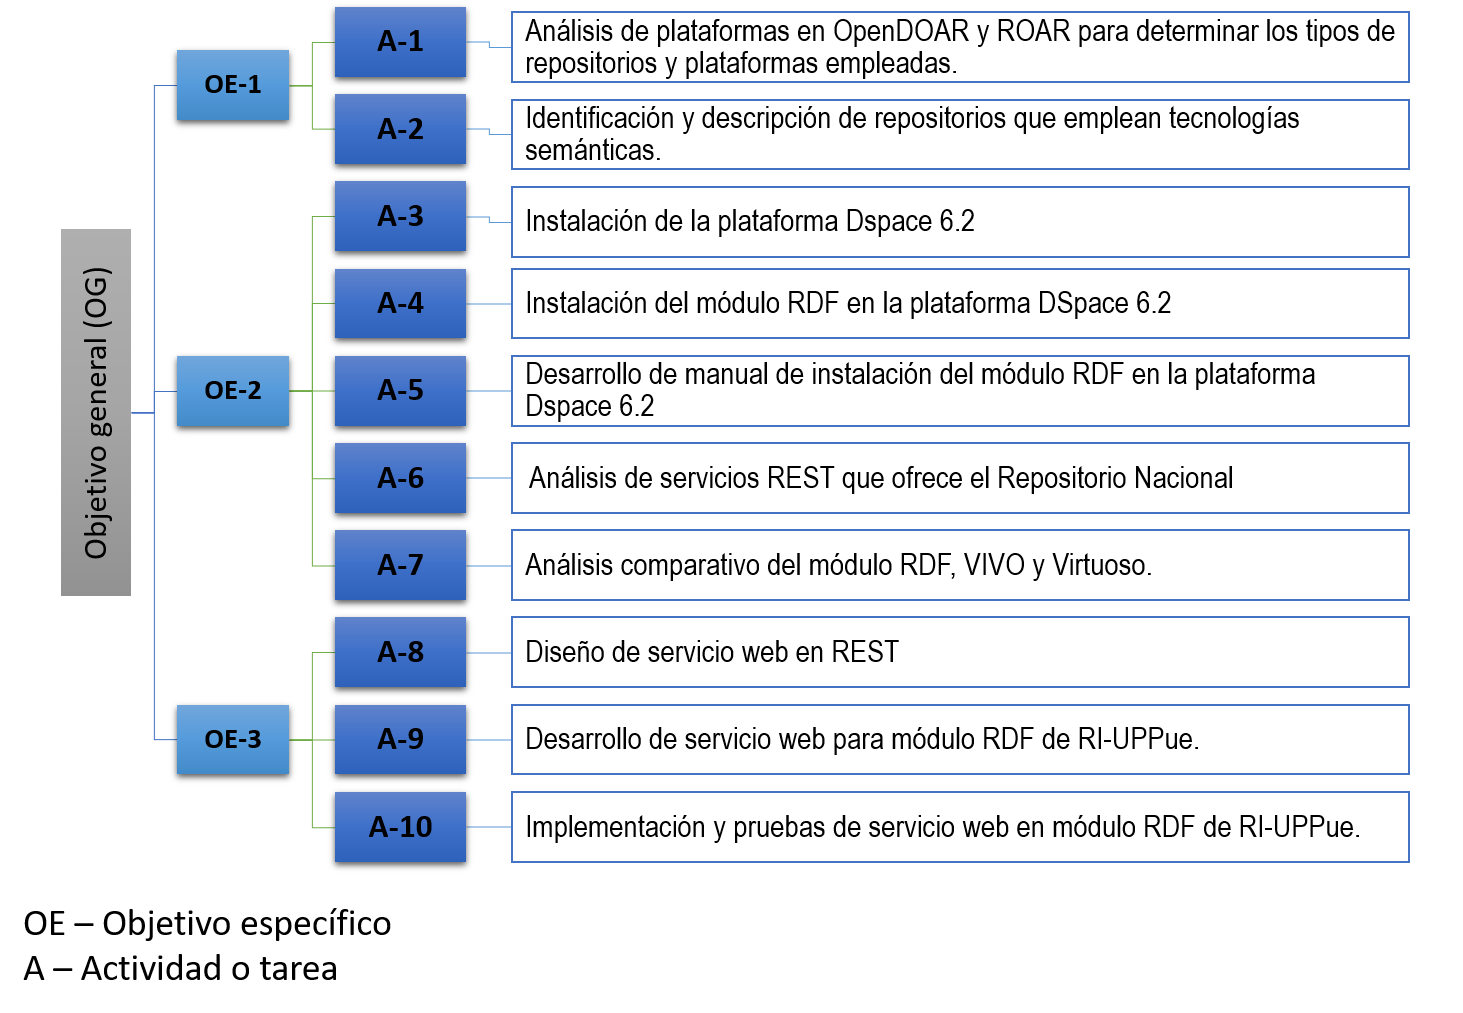
\includegraphics[width=12cm]{figures/Actividades_Dic_2018.png} %NOMBRE DE LA FIGURA y TAMANIO
%%    \caption{Tareas a desempe\~{n}ar para el desarrollo del servicio web} %PIE DE LA IMAGEN
%%    \label{actividades_objetivos}
%%\end{figure}

\section{Justificaci\'on}

En los \'ultimos a\~{n}os, diferentes IES, CIs y comunidades se han sumado el esfuerzo de promover el AA a sus contenidos cient\'ificos mediante RIs que en su mayor\'ia emplea modelos de datos relacionales para almacenar informaci\'on. De acuerdo con \cite{ASWebQuest}  y \cite{GuideCreatingOntology}, el uso de tecnolog\'ias sem\'anticas como las ontolog\'ias se caracteriza por lo siguiente: 

\begin{itemize}
\item Intercambio de datos entre aplicaciones, programas y/o plataformas mediante el lenguaje XML\footnote{XML son las siglas de \textit{eXtensible Markup Language}}  o lenguajes derivados de \'este
\item Las ontolog\'ias permiten gestionar datos incompletos y reutilizar el conocimiento 
\item Los datos en las ontolog\'ias forman conjuntos de datos que son procesables por computadora

\end{itemize}

Los beneficios esperados del desarrollo de la tesis son:
	
	\begin{itemize}
	 \item Recopilaci\'on y divulgaci\'on de datos de producci\'on cient\'ifica y acad\'emica del RI-UPPue en formatos de la web sem\'antica    
         \item Uso de la ontolog\'ia Onto4AIR como alternativa de integraci\'on de informaci\'on sem\'antica a datos provenientes de otros RIs
         \item Extensi\'on de los mecanismos de b\'usqueda y recuperaci\'on del RI-UPPue, recuperaci\'on desde un punto de vista conceptual y no s\'olo textual 
         \end{itemize}


    \part{Marco teórico}
	\renewcommand{\chaptername}{Cap\'itulo}
\chapter{Marco Te\'orico} 
\label{MarcoTeorico}

El cap\'titulo \ref{MarcoTeorico} se organiza como sigue: en primer lugar trata la importancia de los metadatos, considerados como datos descriptivos para los documentos de los repositorios. Posteriormente, se presenta el modelo de datos RDF y su contexto en la web sem\'antica, seguido de una breve descripci\'on del lenguaje de consulta est\'andar para datos en RDF, SPARQL. En la tesis, el acceso a los datos se implementa en servicios REST, por lo que se describen sus caracter\'isticas principales junto con los requerimientos para repositorios de acuerdo con la  \emph{Confederation of Open Access Repositories},  Confederaci\'on de Repositorios de Acceso Abierto (COAR). Finalmente, el cap\'titulo describe los trabajos relacionados. 

\section{La importancia de los metadatos}

Actualmente, en la web existe gran cantidad de informaci\'on sobre cualquier tema, tanta que se requiere del desarrollo de servicios que consideren su pertinencia, veracidad y  calidad para satisfacer necesidades de informaci\'on espec\'ificas de los usuarios tomando en cuenta aspectos t\'ecnicos de accesibilidad y disponibilidad, esto porque el acceso se realiza desde cualquier lugar y mediante una gama amplia de dispositivos.\newline

El etiquetado y descripci\'on de los contenidos son cruciales en el desarrollo de ese tipo de servicios, el primero permite categorizar o clasificar, el segundo se refiere al uso de las descripciones, elementos descriptores o \emph{metadatos} para que los recursos digitales se localicen y procesen adecuadamente por agentes tales como computadoras, aplicaciones m\'oviles y usarios con roles y caracter\'isticas propias. \newline

Seg\'un \cite{W3C}, una prio\-ri\-dad particular del \emph{World Wide Web Consortium}, (Consorcio W3C), es usar la web para documentar el significado de los metadatos. La importancia de la gesti\'on, uso y representaci\'on de los metadatos en modelos sem\'anticos u ontolog\'ias, se relaciona directamente con el modelo de datos conocido como Marco de Descripci\'on de Recursos, en ingl\'es \emph{Resource Description Framework}, (RDF). La secci\'on \ref{RDF} describe caracter\'isticas de este modelo junto con otras tecnolog\'ias de la web sem\'antica.\newline

\section{RDF en el contexto de la web sem\'antica}
\label{RDF}

La web es una plataforma tecnol\'ogica que constituye la mayor base de datos existente, se conforma por todo tipo de recursos, donde las personas o usuarios realizan tareas como publicar, explorar, consultar, almacenar datos e informaci\'on. En sus inicios, en la web se consideraba que los recursos debieran ser entendidos s\'olo por los usuarios, con el paso del tiempo y la gran cantidad de datos que est\'an en ella, es de suma importancia su gesti\'on y procesamiento mediado por las computadoras. \newline

La web sem\'antica, extensi\'on de la web tradicional, promueve el modelado, etiquetado y representaci\'on de la informaci\'on de manera que tanto los humanos como las computadoras sean capaces de ``comprender'' el contenido y la descripci\'on de los recursos; como menciona \cite{IntroBDRDF}, esta web propone una alternativa para agregar significado a los contenidos almacenados con el prop\'osito de propiciar una interacci\'on m\'as fluida entre aplicaciones, servicios, computadoras y el ser humano en comparaci\'on con la web tradicional. \newline

Las tecnolog\'ias de la web sem\'antica se rigen bajo ciertas normas y lenguajes est\'andar organizados en capas o niveles, como muestra la figura \ref{ModeloWebSemantica}, los cuales se describen a continuaci\'on \cite{IntroBDRDF}:

\begin{figure}[!ht]
    \centering
    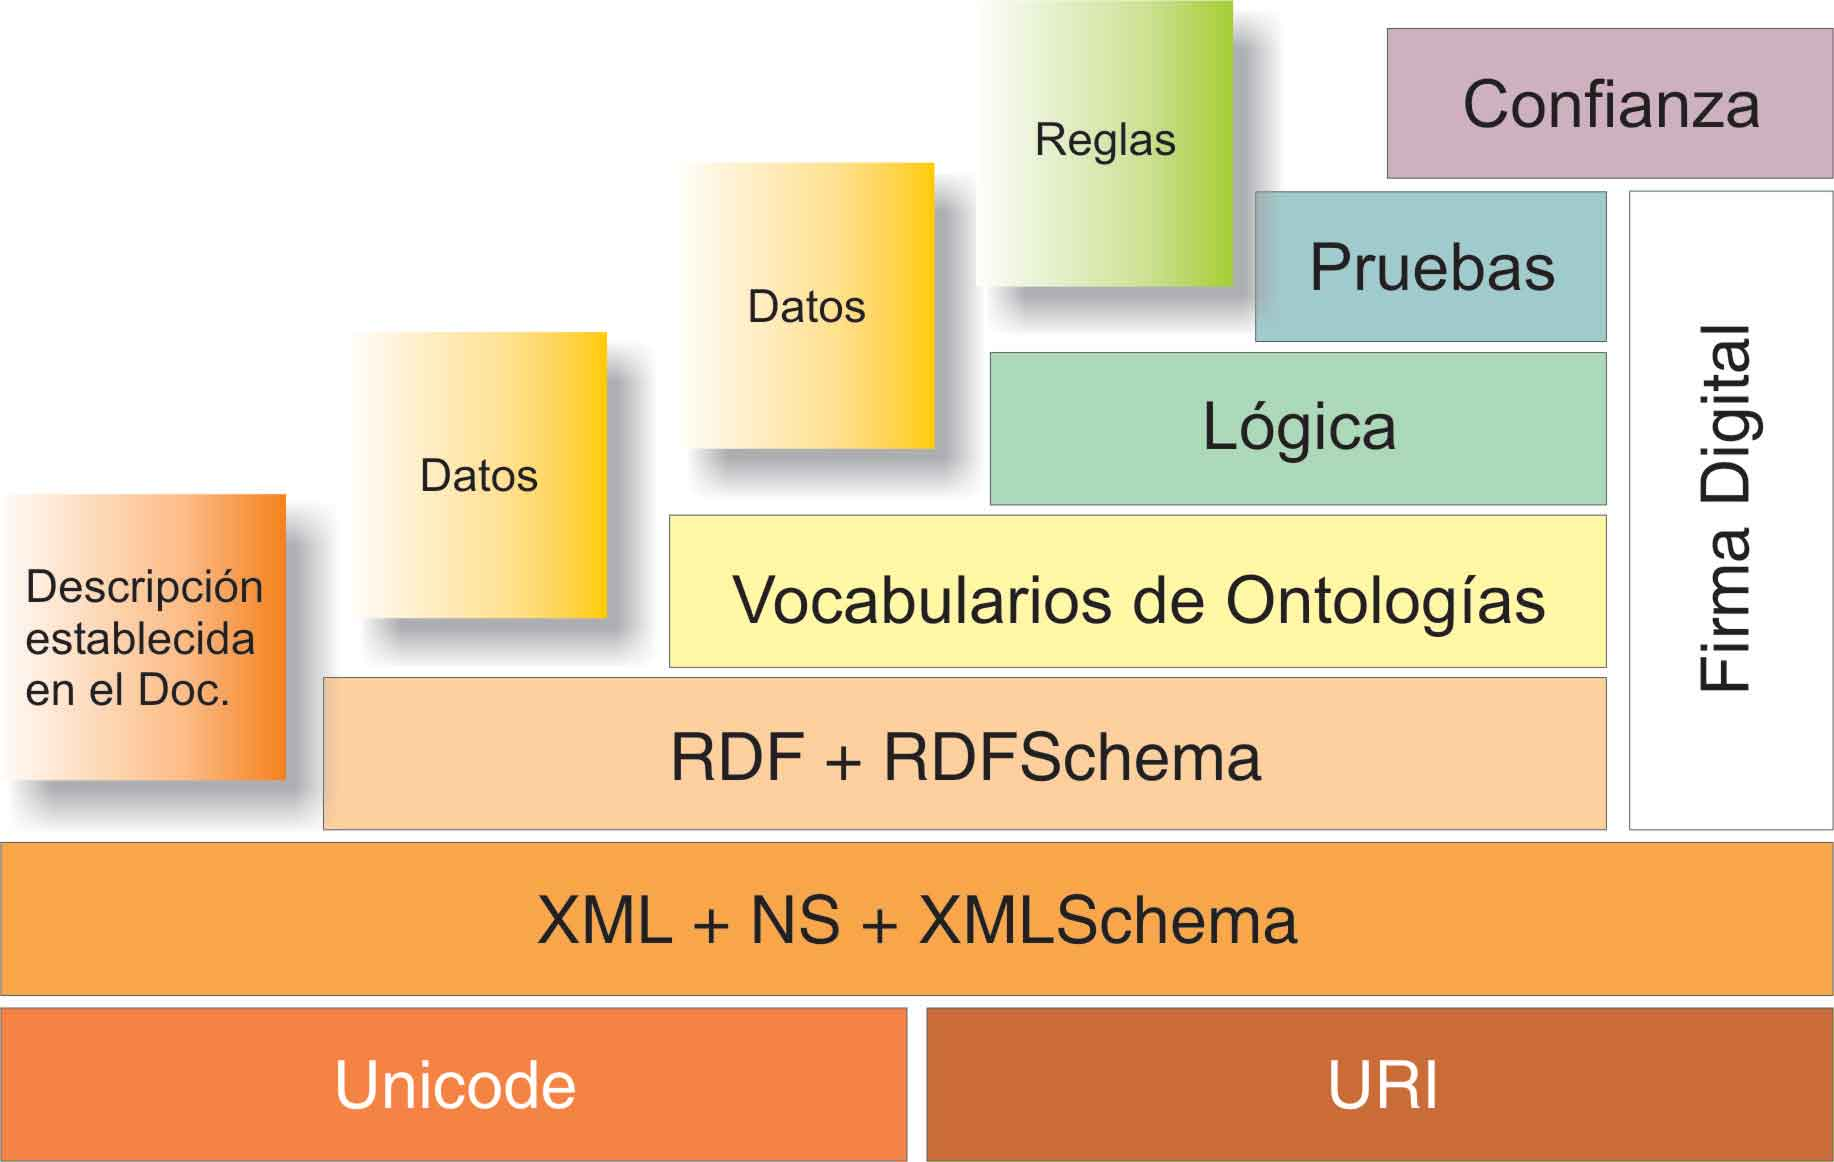
\includegraphics[width=10cm]{figures/ModeloCapasWebSemantica.jpg} %NOMBRE DE LA FIGURA y TAMAÑO
    \caption{Modelo de capas de Berners-Lee para la web sem\'antica\cite{WebSemanticaSciELO}} %PIE DE LA IMAGEN
    \label{ModeloWebSemantica}
\end{figure}

\begin{itemize}
    \item \textit{Unicode} \cite{W3C}. Est\'andar para documentos de texto que permite codificar la mayor\'ia de los sistemas de escritura del mundo.
    
    \item \textit{Uniform Resource Identifier}, (URI), identificador uniforme de recursos \cite{W3C}. Es\-t\'an\-dar para crear identificadores de recursos web a trav\'es de cadenas compactas de ca\-rac\-te\-res, identifican a los recursos de forma un\'ivoca, se emplean para localizarlos de forma autom\'atica. Un \textit{Uniform Resource Locator}, (URL), identificador de recursos uniforme, es un tipo de URI, por ejemplo, \texttt{http://informatica.uppuebla.edu.mx/} identifica espec\'ificamente a la p\'agina inicial de un servidor. 

    \item \textit{XML\footnote{\textit{eXtensible Markup language} (Lenguaje de Marcado Extensible o Lenguaje de Marcas Extensible)}} \cite{W3C}. Es un lenguaje de marcado similar a HTML, es una especificaci\'on del W3C de prop\'osito general en la que cada usuario define sus propias etiquetas. 
    
    \item \textit{XML namespaces} \cite{W3C}. Los espacios de nombre de XML se emplean para atender el problema de ambig\"{u}edad en los documentos XML de la web, de manera que cada elemento est\'a identificado por una URI que lo hace \'unico y universal. Los espacios de nombre son recomendaci\'on de W3C.
    
    \item RDF \cite{W3CSemanticWeb}. Modelo est\'andar para el intercambio de datos en la web, con caracter\'isticas que facilitan la fusi\'on de datos incluso en diferentes esquemas. RDF ampl\'ia la estructura de enlaces web (\emph{links}) para nombrar a dos recursos denominados \emph{sujeto} y \emph{objeto}, as\'i como a la relaci\'on entre ellos. Estos enunciados se conocen como \textit{ternas} o \emph{tripletas}. En el modelo de datos RDF se representan datos estructurados y semiestructurados o combinaciones, estos datos se comparten y utilizan por diferentes aplicaciones.
    
    \item \textit{RDF Schema} \cite{W3CRDFSchema}. Proporciona un vocabulario para el modelo de datos RDF, lo complementa con diferentes documentos anexos que describen los conceptos b\'asicos y la sintaxis abstracta de RDF. RDF Schema es una extensi\'on sem\'antica de RDF que proporciona mecanismos para describir grupos de recursos y sus relaciones, est\'a escrito en RDF, los recursos se utilizan para determinar las caracter\'isticas de otros recursos como dominio y rango de propiedades.
    
    
    \item \textit{Ontolog\'ia}. Seg\'un \cite{Ontologias}, una ontolog\'ia es un marco com\'un o una estructura conceptual sistematizada y de consenso no s\'olo para almacenar la informaci\'on, sino tambi\'en para poder buscarla y recuperarla. Una ontolog\'ia define los t\'erminos y las relaciones b\'asicas para la compresi\'on de un \'area del conocimiento o dominio, as\'i como las reglas para combinar los t\'erminos que definen las extensiones de este vocabulario controlado
    
    \item \textit{Vocabularios de ontolog\'ias}. El lenguaje de ontolog\'ias web, (\textit{Ontologies Web Language}), est\'a dise\~{n}ado para ser usado en aplicaciones que necesitan procesar el contenido de la informaci\'on,  cuenta con un vocabulario m\'as extenso al de RDF y RDF Schema, junto con una sem\'antica formal. OWL tiene tres sublenguajes que var\'ian por su nivel de expresividad: OWL Lite, OWL DL y OWL Full \cite{LaWebSemantica}
    
    \item \textit{Capa l\'ogica}. Permite determinar si la estructura de los razonamientos es v\'alida a trav\'es del estudio de las reglas formales. En esta capa se infiere conocimiento, requiere de la interacci\'on entre las ontolog\'ias y agentes de software, (programas o aplicaciones) \cite{LaWebSemantica}
    
    \item \textit{Capa de pruebas}. A trav\'es de demostraciones matem\'aticas se comprueba que el procesamiento del agente de software alcance la m\'axima confiabilidad en sus razonamientos \cite{LaWebSemantica}
    
    \item \textit{Capa de confianza}. Establece las pol\'iticas de seguridad que permitan asignar niveles de fiabilidad a determinados recursos, de forma comprobable por agentes. Esta capa usa firmas digitales y redes de confianza \cite{LaWebSemantica}

\end{itemize}

Los lenguajes utilizados ampliamente para representar los datos en la web sem\'antica son XML, RDF y OWL. El lenguaje de consulta para datos en RDF se describe en la secci\'on \ref{SPARQL}.

\section{SPARQL: lenguaje de consulta para datos en RDF}
\label{SPARQL}

RDF es un modelo de datos que se asocia con diferentes representaciones, una de ellas es como un modelo de grafos dirigidos etiquetados que representan informaci\'on en la web. Se emplea para representar informaci\'on personal, datos de redes sociales, metadatos sobre objetos digitales o como medio para la integraci\'on de fuentes de informaci\'on heterog\'eneas.\newline

Los datos en RDF se recuperan utilizando SPARQL, \textit{SPARQL protocol and RDF query language}, protocolo y lenguaje de consulta para RDF, sirve para extraer la informaci\'on contenida en una ontolog\'ia RDF, devuelve resultados en forma de enlaces o esquemas RDF. Entre sus especificaciones, de acuerdo con \cite{SkosSparql}, se encuentran las siguientes:

\begin{itemize}
    \item La especificaci\'on del protocolo SPARQL para RDF \textit{SPROT} que define el protocolo remoto para enviar consultas SPARQL y recibir los resultados
    \item La especificaci\'on del formato XML de los resultados de consultas SPARQL \textit{RESULTS}, define un formato de documento XML para representar los resultados de las consultas \texttt{SELECT} y \texttt{ASK} 
\end{itemize}

La Figura \ref{ejemploRDFgrafico} muestra una representaci\'on gr\'afica simple de \textit{vc-db-1.rdf}, archivo que contiene RDF para varias descripciones de vCard de personas, descritas en las notas del W3C ``Representaci\'on de objetos vCard en RDF / XML''.\newline

\begin{figure}[!ht]
    \centering
    \fbox{
    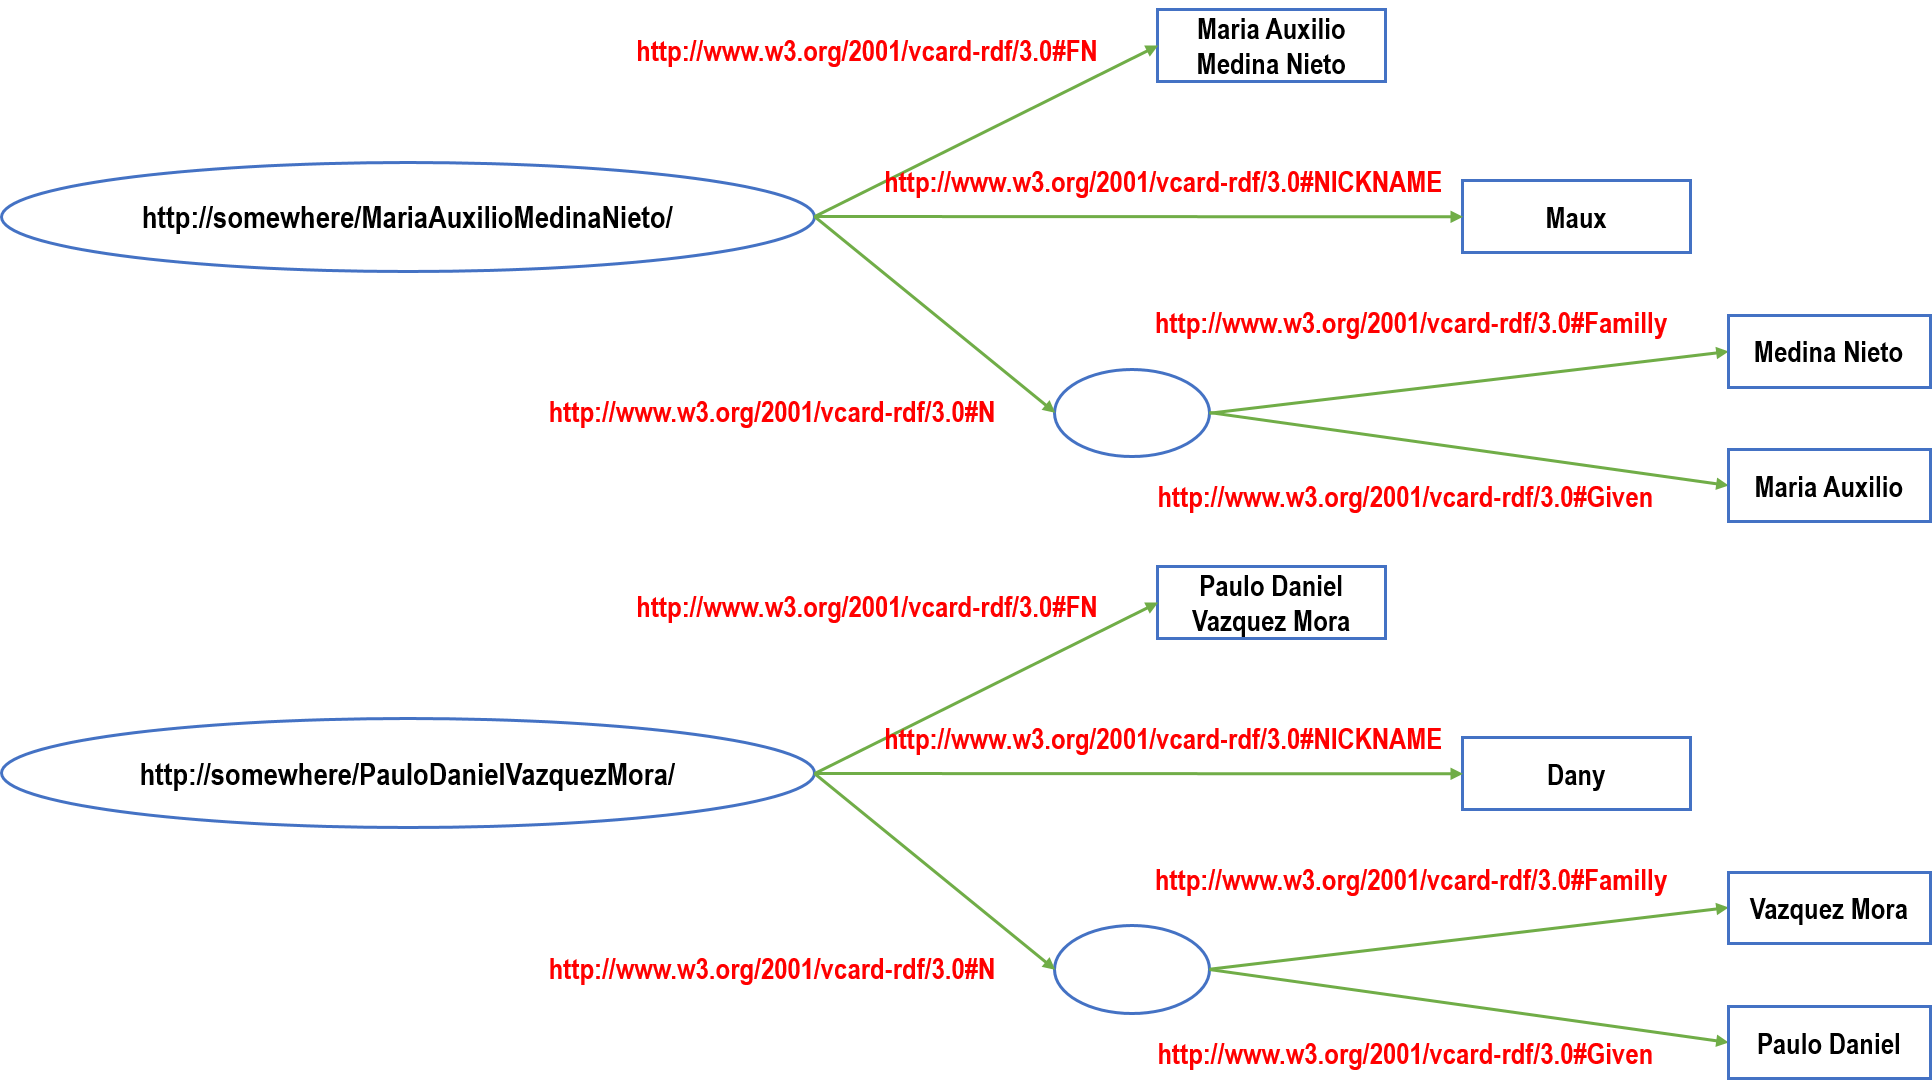
\includegraphics[scale=.44]{figures/vcdb.png}} 
    \caption{Ejemplo de representaci\'on gr\'afica provenientes de objetos vCard en RDF / XML} 
    \label{ejemploRDFgrafico}
\end{figure}

La Figura \ref{ejemploRDF} muestra el esquema RDF expresado como un conjunto de ternas, (tambi\'en llamadas tripletas).\newline

\begin{figure}[!ht]
    \centering
    \fbox{
    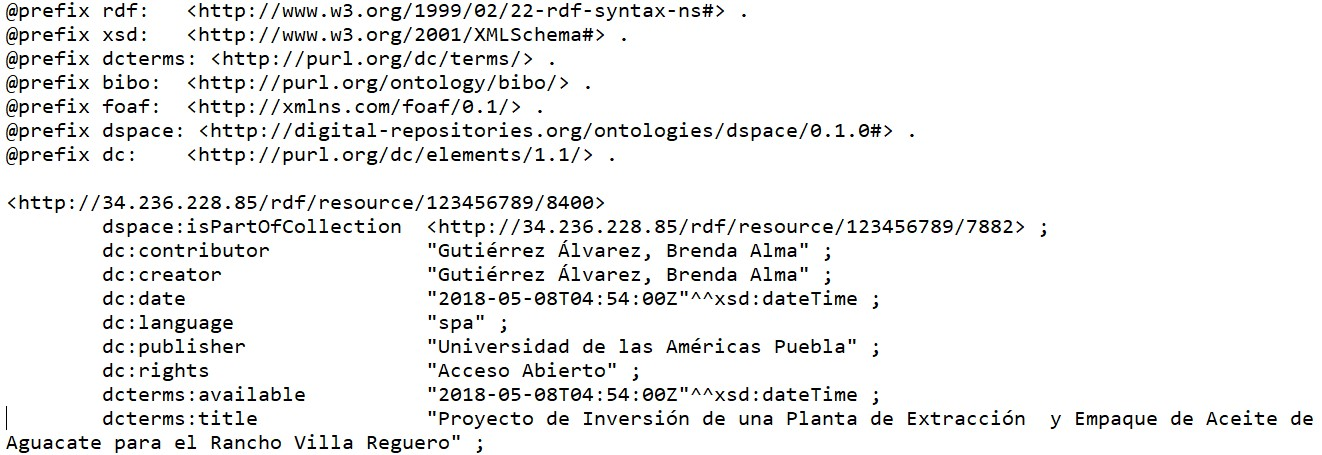
\includegraphics[scale=.45]{figures/ejemploRDF.jpg}} %NOMBRE DE LA FIGURA y TAMAÑO
    \caption{Ejemplo de conjunto de ternas en RDF} %PIE DE LA IMAGEN
    \label{ejemploRDF}
\end{figure}

    
\section{Servicios REST}

Los servicios REST se emplean para explotar recursos a partir de la migraci\'on a la web 2.0, sustituyen aquellos que hac\'ian uso de los protocolos SOAP y WSDL, su arquitectura es sencilla y est\'a orientada a recursos, hacen uso del protocolo HTTP. Los servicios \textit{Re\-pre\-sen\-ta\-tio\-nal State Transfer}, Transferencia de Estado Representacional (REST) cumplen con las premisas siguientes \cite{FeaturesREST}:

\begin{itemize}
    \item Se define una \emph{interfaz} de comunicaci\'on \emph{cliente-servidor} que separa las res\-pon\-sa\-bi\-li\-da\-des entre ambas partes como muestra la figura \ref{arquitecturaREST1}.
    
        \begin{figure}[!ht]
        \centering
        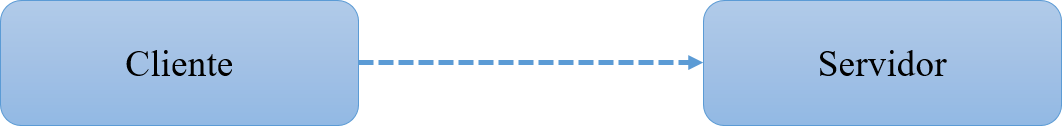
\includegraphics[width=10cm]{figures/ClienteServidorREST.png} 
        \caption{Arquitectura cliente servidor de servicio REST} 
        \label{arquitecturaREST1}
    \end{figure}

 \item Servicio web \emph{sin estado} ya que  cada petici\'on que se realiza es completamente independiente de cualquier otra, sin embargo, todas las solicitudes al mismo servicio son id\'enticas,  ver la Figura \ref{arquitecturaREST2}.
    
    \begin{figure}[!ht]
        \centering
        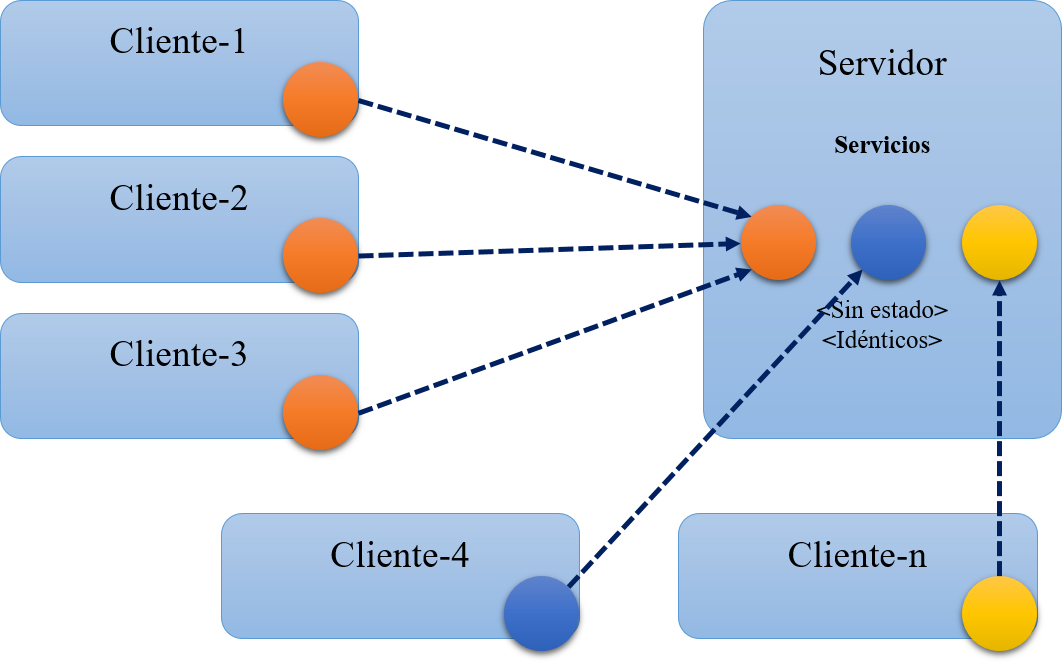
\includegraphics[width=10cm]{figures/ClienteServidorREST2.png} %NOMBRE DE LA FIGURA y TAMAÑO
        \caption{Servicios sin estado de la arquitectura cliente servidor REST} %PIE DE LA IMAGEN
        \label{arquitecturaREST2}
    \end{figure}
    
    \item Los servicios web tipo REST pueden guardar en cach\'e su contenido de tal manera que una vez realizada la primera petici\'on, el resto de peticiones puedan apoyarse en la cach\'e si fuera necesario,  ver la Figura \ref{arquitecturaREST3}.
    
    \begin{figure}[!ht]
        \centering
        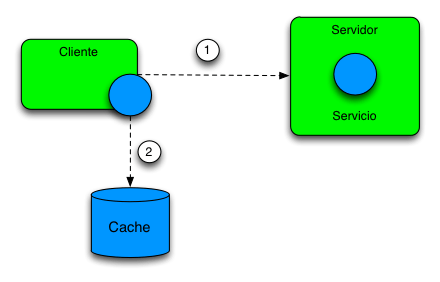
\includegraphics[width=10cm]{figures/ClienteServidorREST3.png} %NOMBRE DE LA FIGURA y TAMAÑO
        \caption{Servicios REST apoyados en cach\'e} %PIE DE LA IMAGEN
        \label{arquitecturaREST3}
    \end{figure}
    
    \item Todos lo servicios REST son \emph{uniformes}, es decir, comparten una forma de invocaci\'on y m\'etodos \url{GET, POST, PUT, DELETE}, ver la Figura \ref{arquitecturaREST4}.
    
    \begin{figure}[!ht]
        \centering
        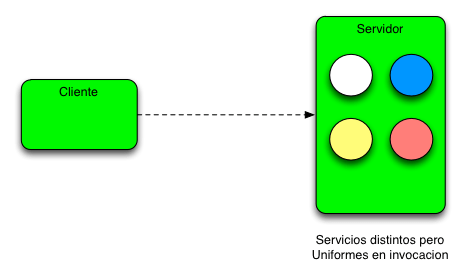
\includegraphics[width=10cm]{figures/ClienteServidorREST4.png} %NOMBRE DE LA FIGURA y TAMAÑO
        \caption{Servicios REST uniformes} %PIE DE LA IMAGEN
        \label{arquitecturaREST4}
    \end{figure}
    
    \item Los servicios REST son escalables y para el cliente transparentes, es decir, el cliente no puede distinguir si la petici\'on es atendida directamente por el servidor o por el sistema de cach\'es debido al servicio de balanceo de cargas, ver la Figura \ref{arquitecturaREST5}.
    
    \begin{figure}[!ht]
        \centering
        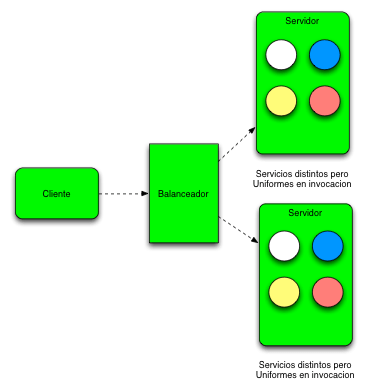
\includegraphics[width=10cm]{figures/ClienteServidorREST5.png} %NOMBRE DE LA FIGURA y TAMAÑO
        \caption{Arquitectura de capas de los servicios REST} %PIE DE LA IMAGEN
        \label{arquitecturaREST5}
    \end{figure}
    
\end{itemize}

Si bien algunos repositorios institucionales (RIs) cuentan con servicios tipo REST, el grado de complejidad en las consultas que hasta el momento est\'an implementadas, consideran s\'olo un atributo o caracter\'istica de los documentos, lo cual restringe el tipo de informaci\'on que puede recuperarse. El RN ofrece un cat\'alogo de m\'as de doscientos servicios REST \footnote{Disponible en: \textit{https://www.repositorionacionalcti.mx/docs/manualesInteroperabilidad}} que estan disponibles para aquellos usuarios que requieren informaci\'on (en formato JSON) \cite{CatalogoRESTRN} de cualquiera de los apartados mostrados en el cuadro \ref{descripcionserviciosRESTRN}.

\begin{table}[htbp]
\caption{Cat\'alogo de servicios REST ofrecidos por el RN} %Leyenda de la tabla
\begin{tabular}{| p{7cm}| p{7cm} |} \hline
\'areas de conocimiento          & Licencia                       \\ \hline
Campos de conocimiento         & Localidad                      \\ \hline
Disciplinas de conocimiento    & Municipio                      \\ \hline
Subdisciplinas de conocimiento & Nivel de acceso                \\ \hline
Audiencia                      & Pa\'is                           \\ \hline
Estado                         & Persona                        \\ \hline
Instituci\'on                    & Formato                        \\ \hline
Idioma                         & Programa                       \\ \hline
Financiador – Programa         & Proyecto                       \\ \hline
\end{tabular}

\label{descripcionserviciosRESTRN}
\end{table}

%El RN cuenta con un cat\'algo de m\'as de doscientos servicios REST que regresan los resultados en formato JSON \cite{CatalogoREST_RN}. La Tabla \ref{descripcionServiciosRESTRN} muestra la descripci\'on general.

%\begin{table}[!ht]
%    \centering
%    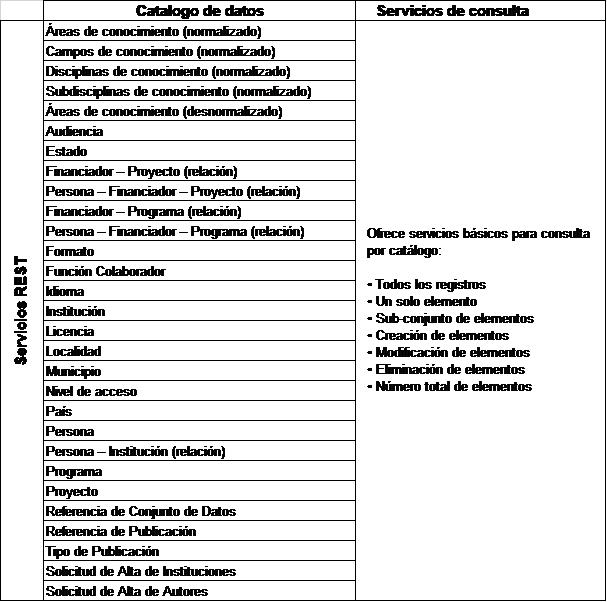
\includegraphics[width=10cm]{figures/TablaServiciosREST.png} %NOMBRE DE LA FIGURA y TAMAÑO
%    \caption{Descripci\'on de los servicios REST ofrecidos por el RN} %PIE DE LA IMAGEN
%    \label{descripcionServiciosRESTRN}
%\end{table}

Dependiendo del cat\'alogo, los servicios se consideran b\'asicos o espec\'ificos. La Figura \ref{ejemploConsumoRESTRN} muestra los elementos principales que intervienen en el consumo de un servicio del RN.\newline

\begin{figure}[!ht]
    \centering
    \fbox{
    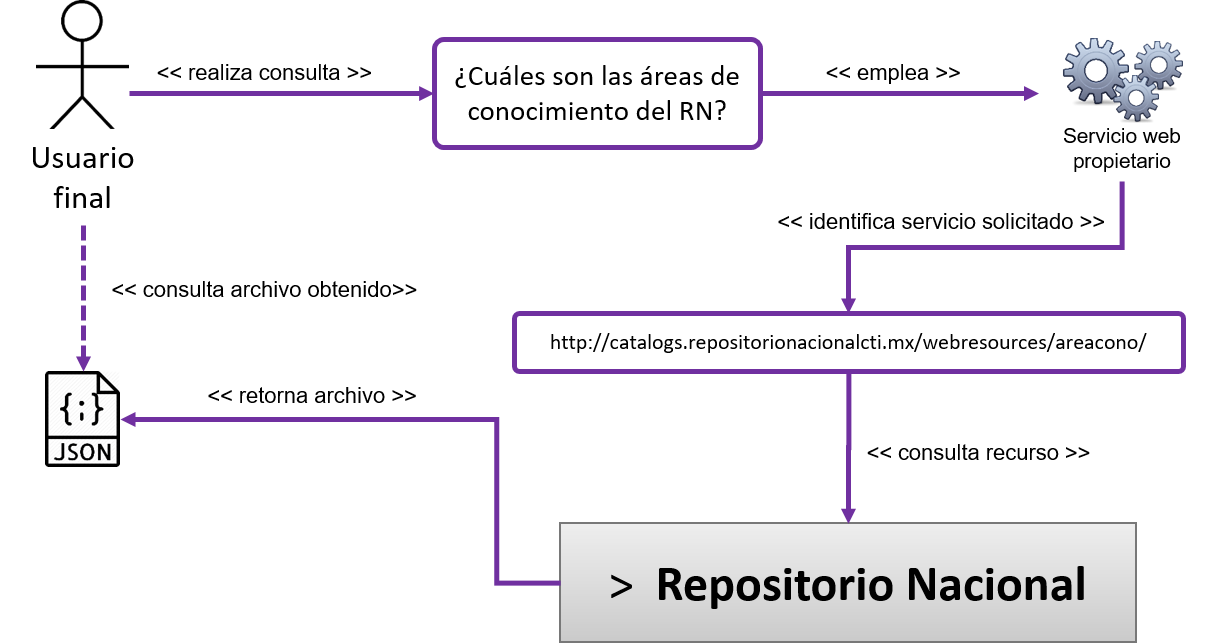
\includegraphics[scale=.75]{figures/ConsumoREST.png}} %NOMBRE DE LA FIGURA y TAMAÑO
    \caption{Ejemplo de consumo de un servicio REST del RN} %PIE DE LA IMAGEN
    \label{ejemploConsumoRESTRN}
\end{figure}

Los resultados de los servicios REST se almacenan en un archivo en formato \textit{JavaScript Object Notation} (JSON), formato de texto ligero utilizado para intercambiar datos. La Figura \ref{JSONejemploConsumoRESTRN} ilustra la manera en que un usuario o un agente consume un servicio REST.\newline

\begin{figure}[!ht]
    \centering
    \fbox{
    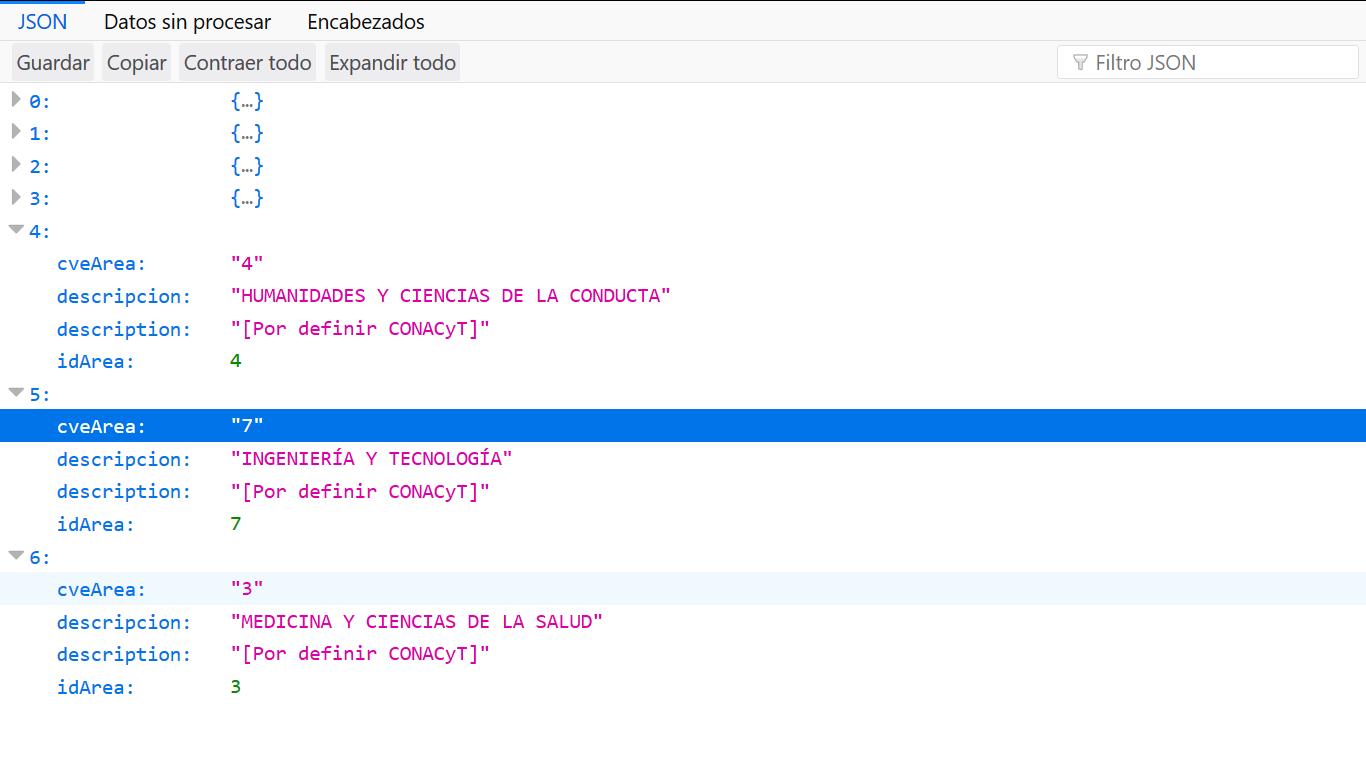
\includegraphics[scale=.45]{figures/JSONservicioRESTRN.png}} %NOMBRE DE LA FIGURA y TAMAÑO
    \caption{Archivo tipo JSON obtenido mediante servicio REST del RN} %PIE DE LA IMAGEN
    \label{JSONejemploConsumoRESTRN}
\end{figure}

El uso del protocolo REST permite el intercambio y manipulaci\'on de datos a trav\'es de Internet, lo cual contribuye al desarrollo de diversas aplicaciones y servicios web que usan datos con diversos or\'igenes. REST funge como interfaz entre un RI que use HTTP para obtener datos o generar operaciones sobre esos datos en formatos como XML y JSON. 

\section{COAR}

Uno de los aspectos que no aportan a la igualdad y libre acceso a la informaci\'on es la publicaci\'on en medios tradicionales, cuyos incentivos coorporativos ponen en desventaja a aquellos que no cuentan con acceso a sus plataformas, medios digitales o impresos. Para las IES y CI que distribuyen documentos en AA, diversos medios han apoyado la difusi\'on de la investigaci\'on y de la producci\'on acad\'emica que se caracterizan por recuperar documentos a partir de palabras clave. En 2016, la \emph{Confederation of Open Access Repositories},  Confederaci\'on de Repositorios de Acceso Abierto (COAR) integr\'o el equipo de trabajo \textit{Next Generation Repository Working Group}, equipo de trabajo para la siguiente generaci\'on de repositorios, cuyo prop\'osito fue definir las funcionalidades y tecnolog\'ias a desarrollar en los RDs en los pr\'oximos a\~{n}os. El informe \textit{Behaviours and Technical Recommendations of the COAR Next Generation Repositories} \cite{NextGenerationRepositories} es resultado de los trabajos, \'este indica que ser\'a necesario adoptar nuevas tecnolog\'ias, est\'andares y protocolos que permitan una mejor integraci\'on de los repositorios en los entornos web, de esta manera, los RDs jugar\'an un papel importante en el amplio campo de la comunicaci\'on acad\'emica. El informe plantea las siguientes caracter\'isticas para que los RDs sean fuentes s\'olidas de publicaci\'on, confiables y de AA \cite{NextGenerationRepositories}:

\begin{itemize}
\item Exponer \textit{identificadores}
\item Declaraci\'on de \textit{licencias} a nivel de recursos
\item Descubrimientos a trav\'es de la \textit{navegaci\'on}
\item Interactuar con \textit{recursos}
\item Descrubrimiento de \textit{lotes}
\item \textit{Transferencia} de recursos
\item \textit{Metadatos} de la actividad de recopilaci\'on y exposici\'on de la informaci\'on
\item \textit{Identificaci\'on} del usuario
\item \textit{Autenticaci\'on} del usuario
\item Exponer \textit{m\'etricas} de uso estandarizadas
\item \textit{Conservaci\'on} de los recursos
\end{itemize}

La visi\'on general del informe marca que, se deben establecer comunidades de investigadores y acad\'emicos que, por un lado, aporten al acervo de los repositorios, por otro lado, que al mismo tiempo incentiven la producci\'on en su comunidad o en otras comunidades interesadas en participar, de tal manera que los repositorios brinden una visi\'on global de la investigaci\'on cient\'ifica y acad\'emica. La tesis propone la implementaci\'on de un servicio web tipo REST conforme a la arquitectura que muestra la Figura \ref{arquitect1} como alternativa tecnol\'ogica acorde con algunos de los elementos del informe.

\begin{figure}[!ht]
    \centering
    \fbox{
    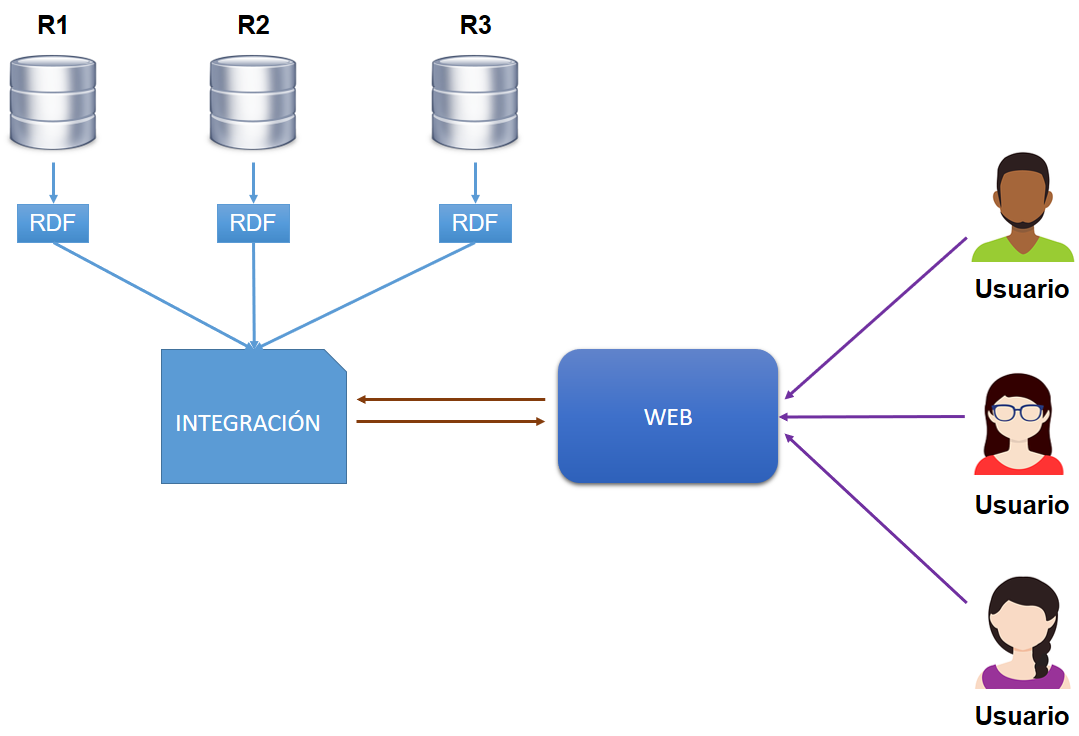
\includegraphics[width=10cm]{figures/ArquitecturaServicioWeb.png}} %NOMBRE DE LA FIGURA y TAMAÑO
    \caption{Arquitectura de servicio web sem\'antico} %PIE DE LA IMAGEN
    \label{arquitect1}
\end{figure}

\section{Trabajos relacionados}

La secci\'on de trabajos relacionados se integra de la revisi\'on documental y de sitios web que abordan tem\'aticas como repositorios, acceso abierto y tecnolog\'ias sem\'anticas. Por ejemplo, \cite{DrJulioSoler} plantea la transferencia de los resultados de investigaci\'on entre universidades o instituciones que, aunque los preservan, generan y transmiten, la transferencia se requiere sea lo m\'as eficiente y efectiva posible, produciendo resultados favorables para los involucrados. Al mismo tiempo, se se\~{n}ala la importancia de la representaci\'on de un dominio adecuado de la gesti\'on de la informaci\'on cient\'ifica definido mediante una ontolog\'ia sobre un software licenciado para la gesti\'on de contenidos (\emph{Content Management System}, sistema de administraci\'on de contenidos (CMS) y contenidos enriquecidos sem\'anticamente.\newline 

La Referencia, Red de Repositorios de Acceso Abierto a la Ciencia \cite{LaReferencia} \footnote{Disponible en: http://www.lareferencia.info/es/}, brinda un espacio para la divulgaci\'on de la ciencia en Latinoam\'erica, incluye en su cat\'alogo repositorios de pa\'ises como Argentina, Brasil, Chile, Colombia, Costa Rica, Ecuador, El Salvador, M\'exico y Per\'u. En los contenidos, los usuarios pueden consultar nodos nacionales, documentos varios, art\'iculos, reportes, tesis de maestr\'ia y doctorado. La Figura \ref{laReferencia} muestra estad\'isticas generales de LA-Referencia. 

\begin{figure}[!ht]
    \centering
    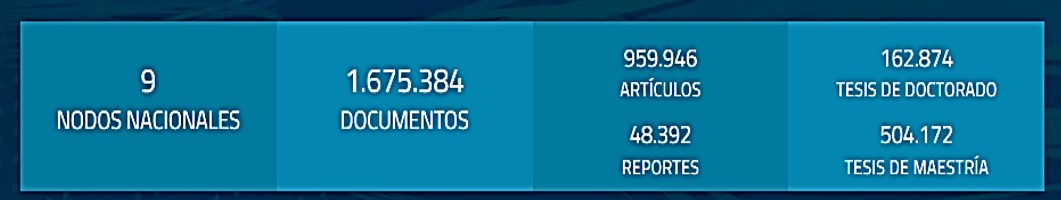
\includegraphics[width=14cm]{figures/lareferencia1.jpg} %NOMBRE DE LA FIGURA y TAMAÑO
    \caption{Estad\'isticas generales reportadas en LA Referencia} %PIE DE LA IMAGEN
    \label{laReferencia}
\end{figure}

OpenDOAR \footnote{Disponible en: http://v2.sherpa.ac.uk/opendoar/} es un directorio global de repositorios de acceso abierto acad\'emico. Permite la identificaci\'on, navegaci\'on y b\'usqueda en funci\'on de una serie de caracter\'isticas de los repositorios como la ubicaci\'on, el software o el tipo de material que se posee. \newline

Al mes de Octubre de 2019, OpenDOAR reporta las estad\'isticas de crecimiento por tipo de plataformas tecnol\'ogicas empleadas por los repositorios de acceso abierto (RAAs), ver Figura \ref{opendoarEstadisticas1}.

\begin{figure}[!ht]
    \centering
    \fbox{
    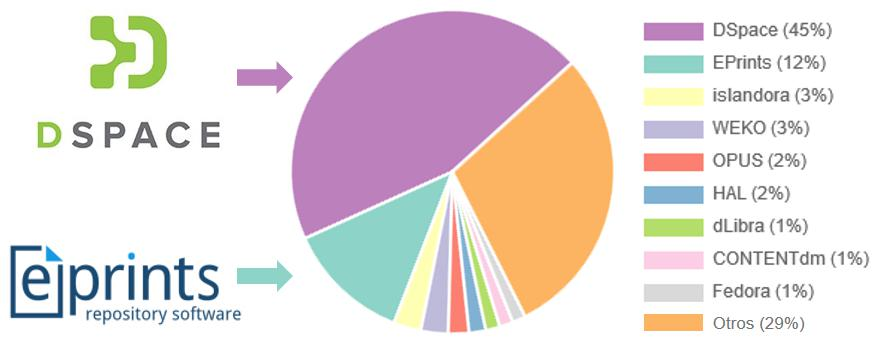
\includegraphics[width=12cm]{figures/opendoar3.jpg}} %NOMBRE DE LA FIGURA y TAMAÑO
    \caption{Repositorios por pa\'is en OpenDOAR} %PIE DE LA IMAGEN
    \label{opendoarEstadisticas1}
\end{figure}

\begin{figure}[!ht]
    \centering
    \fbox{
    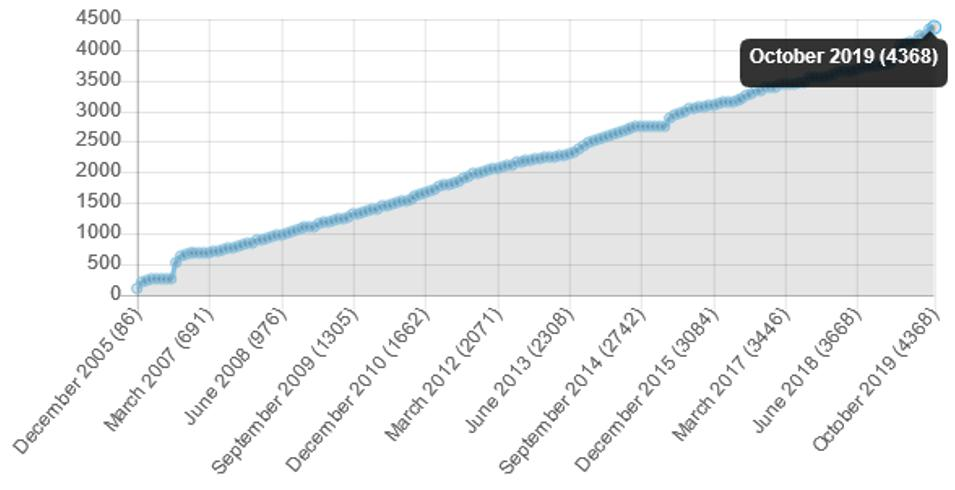
\includegraphics[width=12cm]{figures/opendoar4.jpg}} %NOMBRE DE LA FIGURA y TAMAÑO
    \caption{Repositorios por lenguaje y tipo de software en OpenDOAR} %PIE DE LA IMAGEN
    \label{opendoar_estadisticas_2}
\end{figure}

En Latinoam\'erica, LA Referencia reporta la producci\'on de recursos de AA que muestra la Tabla \ref{produccionRaas} y el tipo de servicios de b\'usqueda disponibles para los usuarios, notar que los atributos recurrentes para las b\'usquedas b\'asicas son: t\'itulo y autor, mientras que en el caso de las avanzadas, el n\'umero de par\'ametros de b\'usqueda var\'ia entre cuatro y doce. Finalmente, se pudo identificar que, ninguno de los repositorios consultados cuenta con  servicio de b\'usqueda sem\'antica.

%\begin{figure}[!ht]
%    \centering
%    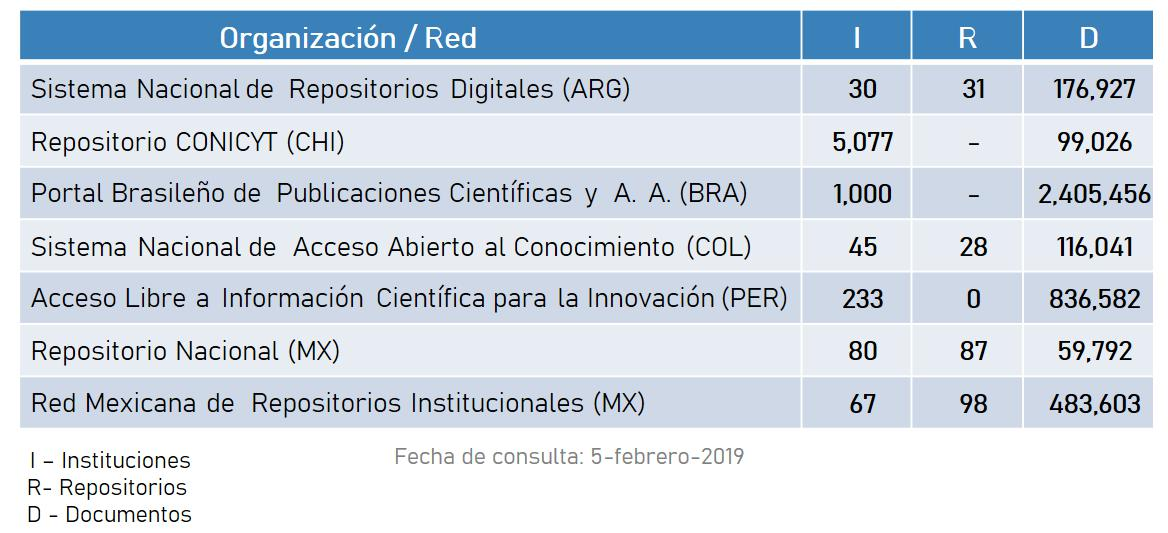
\includegraphics[width=14cm]{figures/estadisticasRaas.jpg}
%    \caption{Repositorios con mayor producci\'on en Latinoam\'erica} %PIE DE LA IMAGEN
%    \label{estadisticasRaas}
%\end{figure}

\begin{table}[htbp]
\caption{Repositorios con mayor producci\'on en Latinoam\'erica}
\begin{tabular}{| p{9.5cm}| p{1.5cm} | p{1.5cm} | p{1.5cm} |}
\hline
\multicolumn{1}{|c|}{\textbf{Organizaci\'on / Red}}                                    & \multicolumn{1}{c|}{\textbf{I}}     & \multicolumn{1}{c|}{\textbf{R}}  & \multicolumn{1}{c|}{\textbf{D}}         \\ \hline
\multicolumn{1}{|l|}{Sistema Nacional de  Repositorios Digitales (ARG)}              & \multicolumn{1}{c|}{\textbf{30}}    & \multicolumn{1}{c|}{\textbf{31}} & \multicolumn{1}{c|}{\textbf{176,927}}   \\ \hline
\multicolumn{1}{|l|}{Repositorio CONICYT (CHI)}                                      & \multicolumn{1}{c|}{\textbf{5,077}} & \multicolumn{1}{c|}{\textbf{-}}  & \multicolumn{1}{c|}{\textbf{99,026}}    \\ \hline
\multicolumn{1}{|l|}{Portal Brasileño de  Publicaciones Cient\'ificas y  A. A. (BRA)}  & \multicolumn{1}{c|}{\textbf{1,000}} & \multicolumn{1}{c|}{\textbf{-}}  & \multicolumn{1}{c|}{\textbf{2,405,456}} \\ \hline
\multicolumn{1}{|l|}{Sistema Nacional de  Acceso Abierto al Conocimiento (COL)}      & \multicolumn{1}{c|}{\textbf{45}}    & \multicolumn{1}{c|}{\textbf{28}} & \multicolumn{1}{c|}{\textbf{116,041}}   \\ \hline
\multicolumn{1}{|l|}{Acceso Libre a Informaci\'on Cient\'ifica para la Innovaci\'on (PER)} & \multicolumn{1}{c|}{\textbf{233}}   & \multicolumn{1}{c|}{\textbf{0}}  & \multicolumn{1}{c|}{\textbf{836,582}}   \\ \hline
\multicolumn{1}{|l|}{Repositorio Nacional (MX)}                                      & \multicolumn{1}{c|}{\textbf{80}}    & \multicolumn{1}{c|}{\textbf{87}} & \multicolumn{1}{c|}{\textbf{59,792}}    \\ \hline
\multicolumn{1}{|l|}{Red Mexicana de  Repositorios Institucionales (MX)}             & \multicolumn{1}{c|}{\textbf{67}}    & \multicolumn{1}{c|}{\textbf{98}} & \multicolumn{1}{c|}{\textbf{483,603}}  \\ \hline
\end{tabular}
\label{produccionRaas}
\footnotesize{ \textbf{\textit{I - Instituciones, R - Repositorios, D - Documentos}}}
\end{table}

%\begin{figure}[!ht]
%    \centering
%    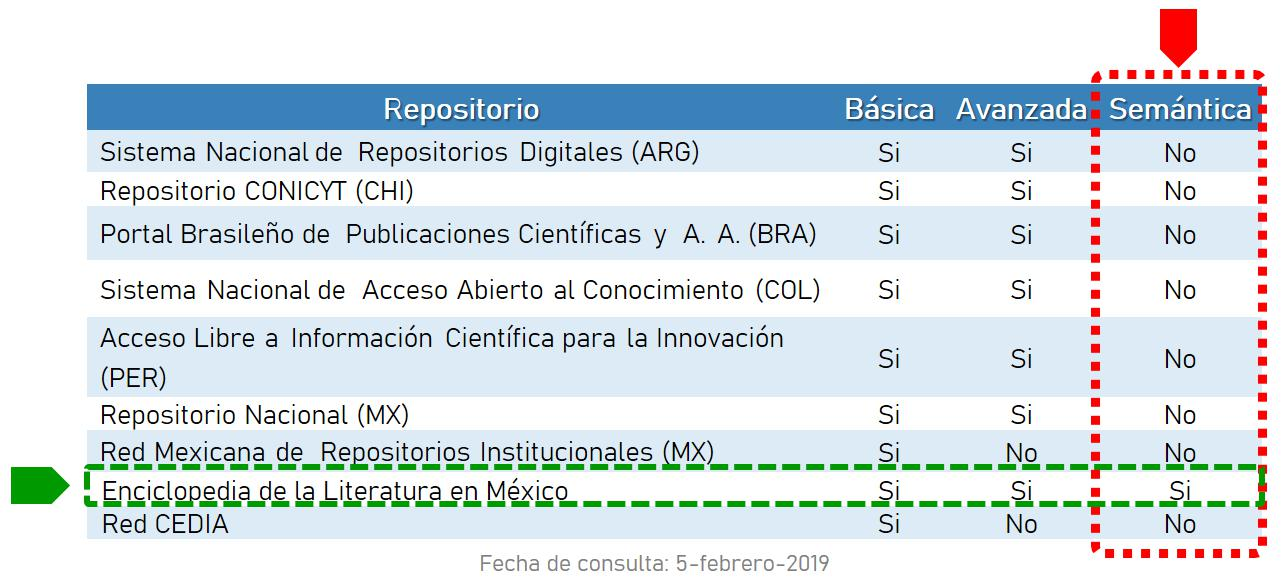
\includegraphics[width=14cm]{figures/serviciosBusquedaSemantica1.jpg} %NOMBRE DE LA FIGURA y TAMAÑO
%    \caption{Servicios de b\'usqueda en RAAs} %PIE DE LA IMAGEN
%    \label{busquedas-raas}
%\end{figure}

\begin{table}[htbp]
\caption{Servicios de b\'usquedas en RAAs}
\begin{tabular}{| p{8.5cm}| p{1.5cm} | p{2cm} | p{2cm} |}
\hline
\multicolumn{1}{|c|}{\textbf{Repositorio}}                     & \textbf{B\'asica} & \textbf{Avanzada} & \textbf{Sem\'antica} \\ \hline
Sistema Nacional de  Repositorios Digitales (ARG)              & Si              & Si                & No                 \\ \hline
Repositorio CONICYT (CHI)                                      & Si              & Si                & No                 \\ \hline
Portal Brasileño de  Publicaciones Cient\'ificas y  A. A. (BRA)  & Si              & Si                & No                 \\ \hline
Sistema Nacional de  Acceso Abierto al Conocimiento (COL)      & Si              & Si                & No                 \\ \hline
Acceso Libre a Informaci\'on Cient\'ifica para la Innovaci\'on (PER) & Si              & Si                & No                 \\ \hline
Repositorio Nacional (MX)                                      & Si              & Si                & No                 \\ \hline
Red Mexicana de  Repositorios Institucionales (MX)             & Si              & No                & No                 \\ \hline
Enciclopedia de la Literatura en M\'exico                        & Si              & Si                & Si                 \\ \hline
Red CEDIA                                                      & Si              & No                & No                 \\ \hline
\end{tabular}
\label{busquedasRaas}
\end{table}

Las figuras \ref{snrd1} a  \ref{alicia-1} muestran las p\'aginas iniciales de los repositorios consultados y secciones de la interfaz correspondientes a sus m\'odulos de b\'usqueda.

\begin{figure}[!ht]
    \centering
    \fbox{
    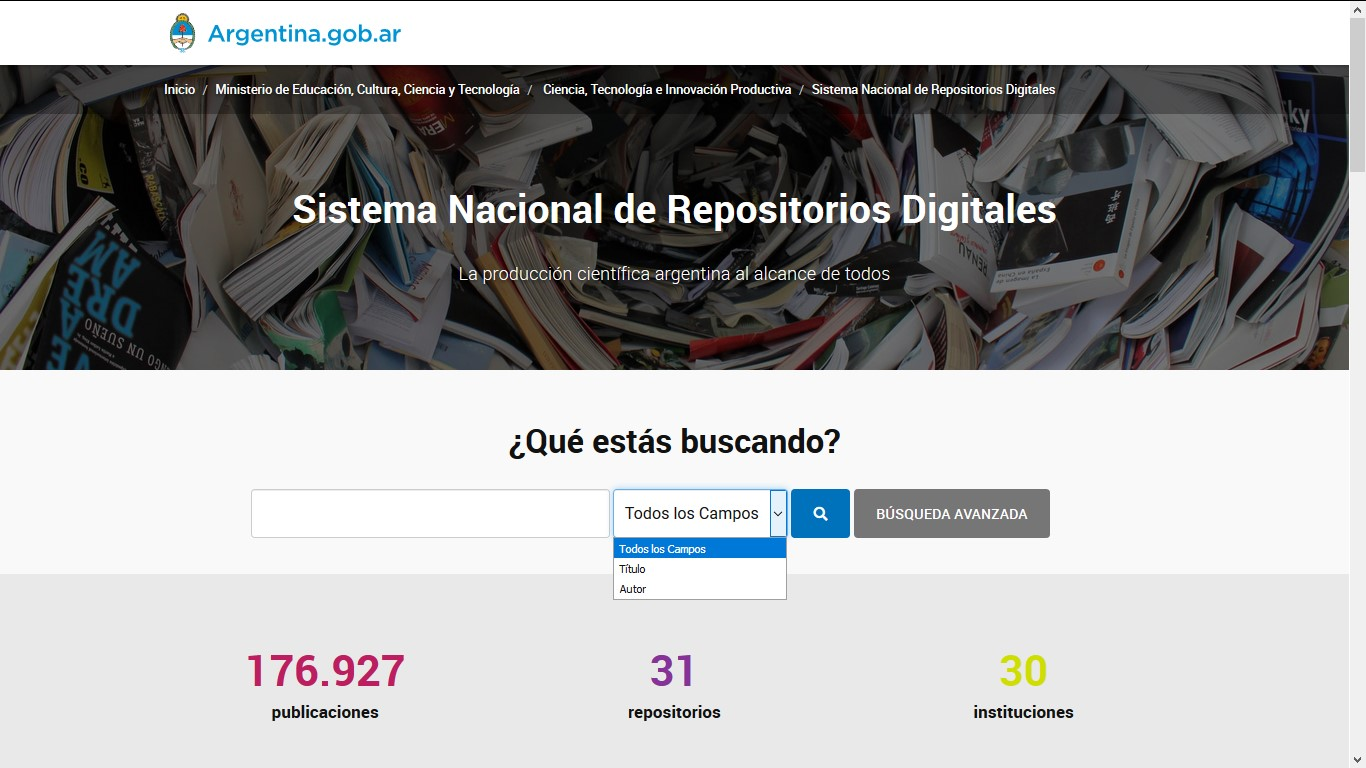
\includegraphics[width=14cm]{figures/repositoriosnrdarg1.jpg}}
    \caption{Vista del portal del Sistema Nacional de Repositorios Digitales} %PIE DE LA IMAGEN
    \label{snrd1}
\end{figure}

\begin{figure}[!ht]
    \centering
    \fbox{
    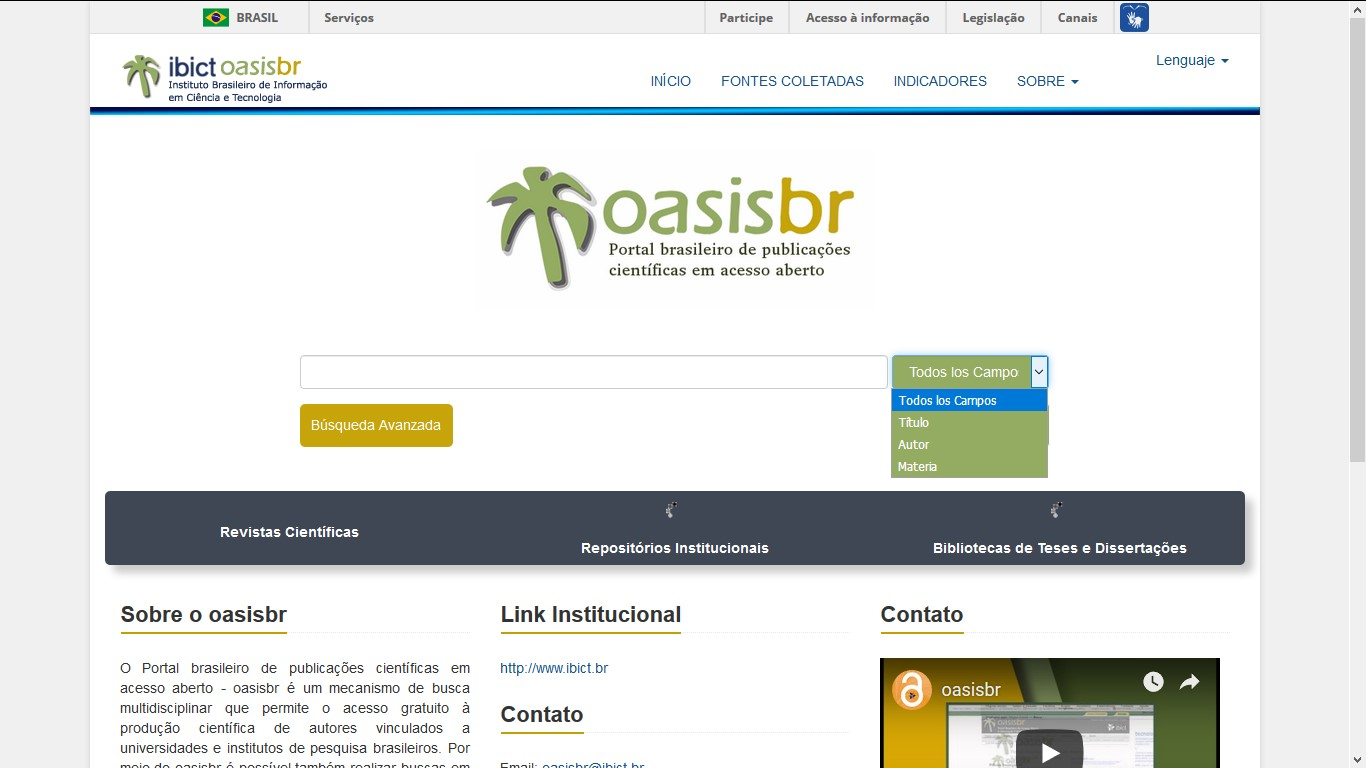
\includegraphics[width=14cm]{figures/repositoriosnrdbr1.jpg}} %NOMBRE DE LA FIGURA y TAMAÑO
    \caption{Vista del portal brasile\~{n}o de publicaciones cient\'ificas y acceso abierto - oasisbr} %PIE DE LA IMAGEN
    \label{oasisbr-1}
\end{figure}

\begin{figure}[!ht]
    \centering
    \fbox{
    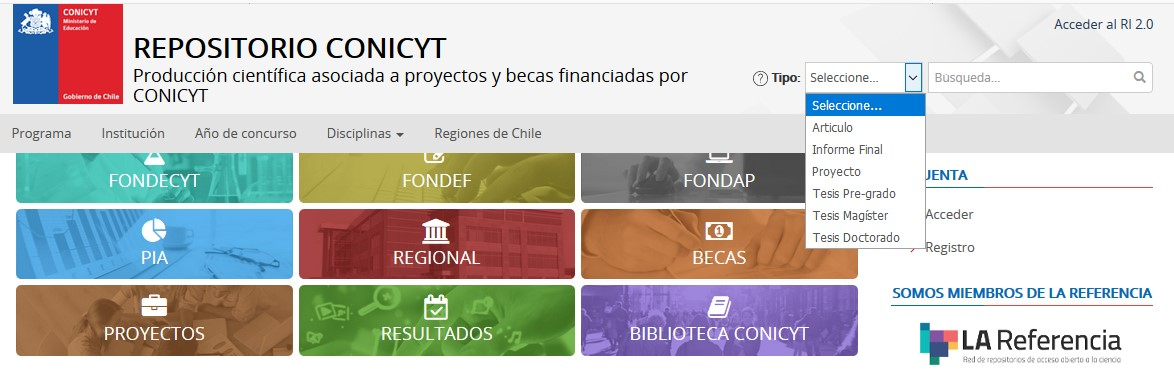
\includegraphics[width=14cm]{figures/repositorioconicytchi3.jpg}} %NOMBRE DE LA FIGURA y TAMAÑO
    \caption{Vista del panel de b\'usquedas en RI2.0} %PIE DE LA IMAGEN
    \label{ri2.0-2}
\end{figure}

\begin{figure}[!ht]
    \centering
    \fbox{
    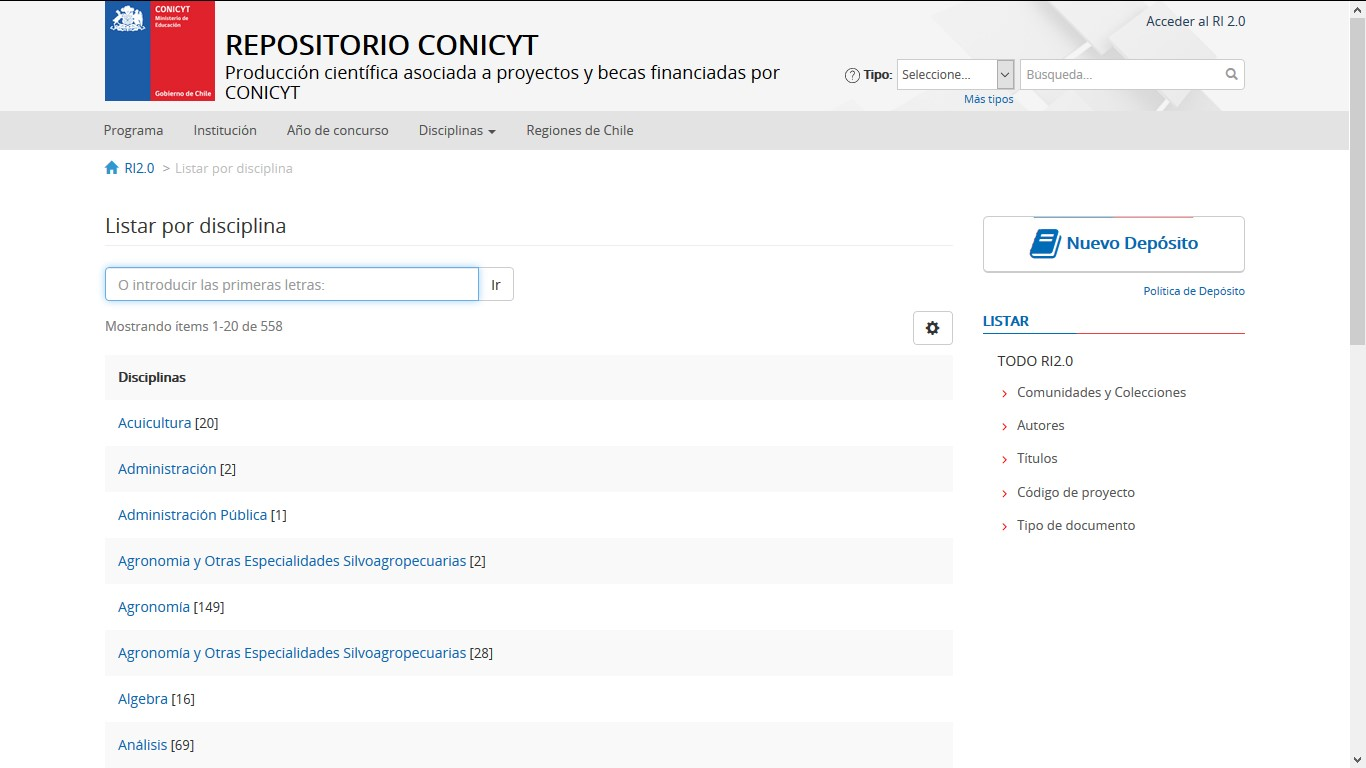
\includegraphics[width=14cm]{figures/repositorioconicytchi2.jpg}} %NOMBRE DE LA FIGURA y TAMAÑO
    \caption{Vista del panel de b\'usquedas avanzadas en RI2.0} %PIE DE LA IMAGEN
    \label{ri2.0-3}
\end{figure}

\begin{figure}[!ht]
    \centering
    \fbox{
    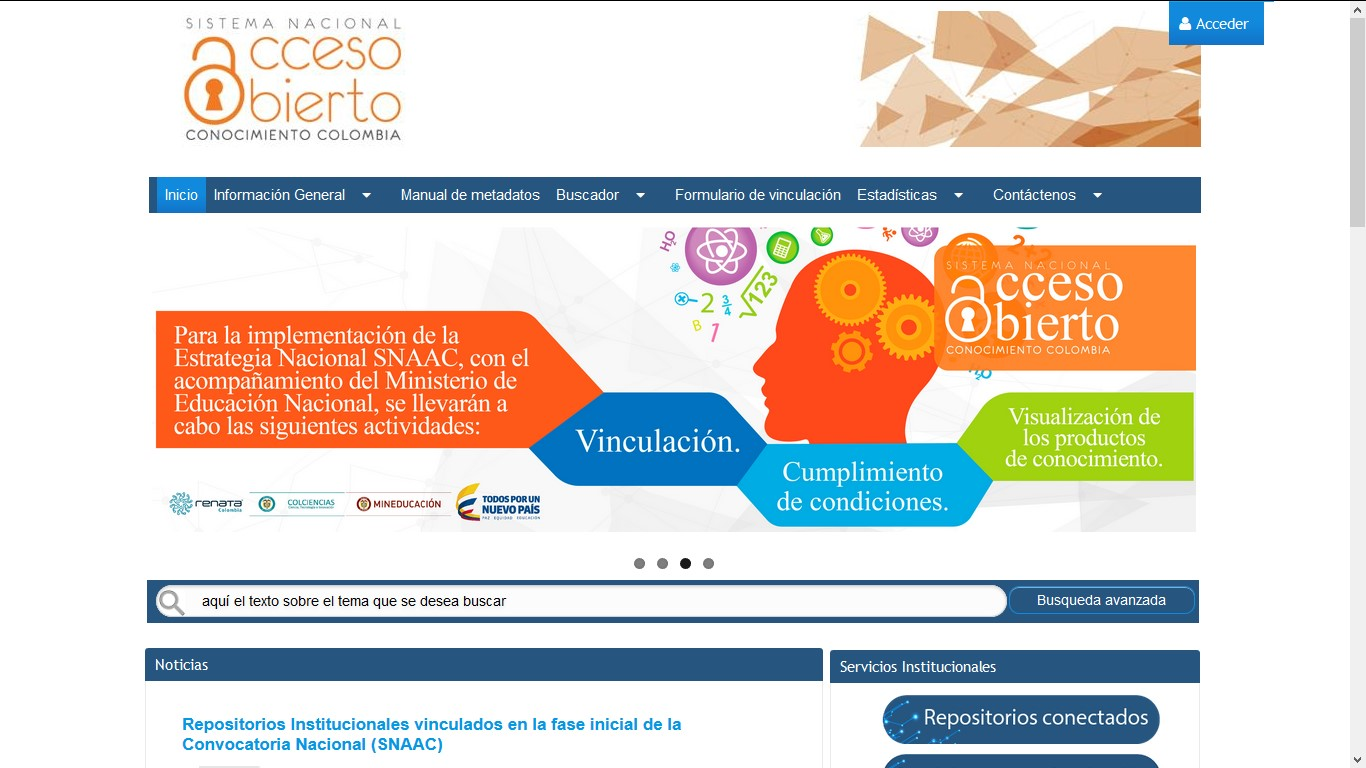
\includegraphics[width=14cm]{figures/repositoriosnaac1.jpg}} %NOMBRE DE LA FIGURA y TAMAÑO
    \caption{Vista del Sistema Nacional de Acceso Abierto al Conocimiento} %PIE DE LA IMAGEN
    \label{snaac-1}
\end{figure}

\begin{figure}[!ht]
    \centering
    \fbox{
    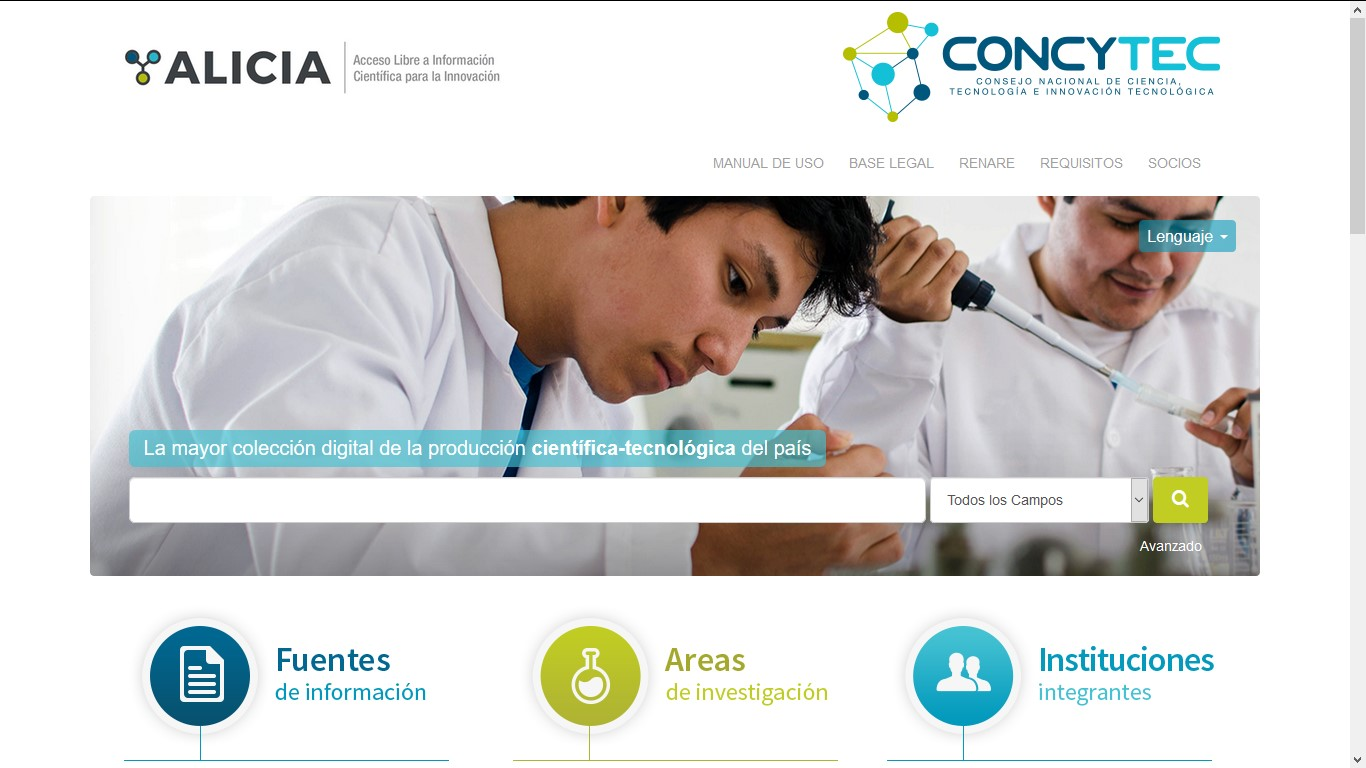
\includegraphics[width=14cm]{figures/repositorioaliciaperu1.jpg}} %NOMBRE DE LA FIGURA y TAMAÑO
    \caption{Vista del portal de acceso libre a informaci\'on cient\'ifica para la innovaci\'on} %PIE DE LA IMAGEN
    \label{alicia-1}
\end{figure}

\subsection{Servicios de b\'usqueda simple, avanzada y sem\'antica}

Las figuras \ref{busquedas-snrd-1} y \ref{busquedas-snrd-2} muestran los servicios de b\'usqueda que ofrecen diferentes RAAs a sus usuarios, basados en criterios de filtrado que en general son comunes tales como el autor, t\'itulo, editor, lenguaje, fecha de publicaci\'on, entre otros.\newline

\begin{figure}[!ht]
    \centering
    \fbox{
    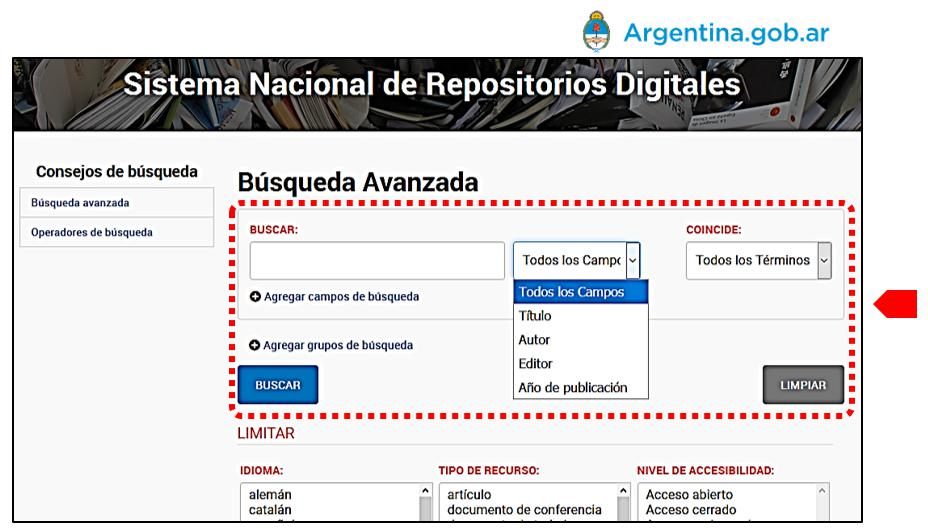
\includegraphics[width=14cm]{figures/BusquedasARG.jpg}} %NOMBRE DE LA FIGURA y TAMAÑO
    \caption{Vista del panel de b\'usqueda en el portal Sistema Nacional de Repositorios Digitales en Argentina} %PIE DE LA IMAGEN
    \label{busquedas-snrd-1}
\end{figure}

\begin{figure}[!ht]
    \centering
    \fbox{
    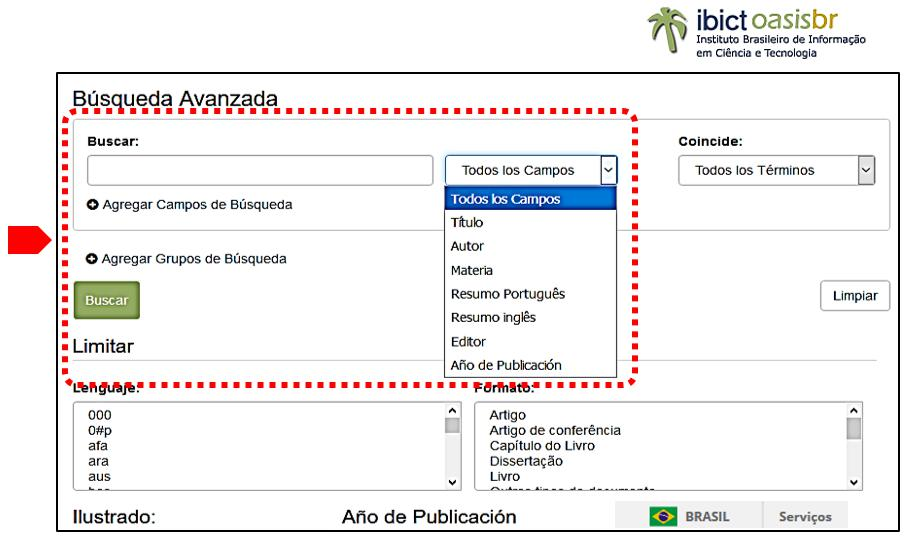
\includegraphics[width=14cm]{figures/BusquedasBRA.jpg}} %NOMBRE DE LA FIGURA y TAMAÑO
    \caption{Vista del panel de b\'usqueda en el portal instituto Brasile\~{n}o de Informaci\'on en Ciencia y Tecnolog\'ia en Brasil} %PIE DE LA IMAGEN
    \label{busquedas-snrd-2}
\end{figure}

La figura \ref{busquedasRaas} concentra informaci\'on de los portales con mayor producci\'on en Latinoam\'erica y los servicios de b\'usqueda que ofrecen, notar que s\'solo uno de los repositorios ofrece servicios basados en tecnolog\'ias sem\'anticas.
\subsection{Comparativa entre plataformas}

Los RAAs cuentan con diversas caracter\'isticas t\'ecnicas que permiten implementar servicios para sus usuarios. Para la implementaci\'on de servicios sem\'anticos se requiere observar tres caracter\'isticas:

\begin{itemize}
    \item Servicio o m\'odulo RDF
    \item Proveedor de almacenamiento de ternas
    \item Lenguaje de consulta
\end{itemize}{}

La tabla \ref{tabla_comparativa} muestra las caracter\'isticas t\'ecnicas entre las plataformas DSpace, Virtuoso y VIVO.\newline

\begin{table}[htbp]
    \begin{center}
    \caption{Tabla comparativa de caracter\'isticas t\'ecnicas entre plataformas DSpace, Virtuoso y VIVO}
    \begin{tabular}{| p{4cm}| p{3cm} |p{4cm} | p{3cm} |}
    \hline
    \centering \textbf{Plataforma} & \textbf{Servicio RDF} & \textbf{Proveedor de almacenamiento} & \textbf{Lenguaje de consulta} \\
    \hline \hline
    DSpace 6.2 & Si & Apache Jena & SPARQL \\ \hline
    Virtuoso & Si & Sesame, Redland, Apache Jena & SPARQL \\ \hline
    VIVO & Si & - & SPARQL \\ \hline
    \end{tabular}
    \label{tabla_comparativa}
    \end{center}
\end{table}

La Figura \ref{ejemploRDFternas} muestra el esquema RDF expresado como un conjunto de ternas, (tambi\'en llamadas tripletas).\newline

\begin{figure}[!ht]
    \centering
    \fbox{
    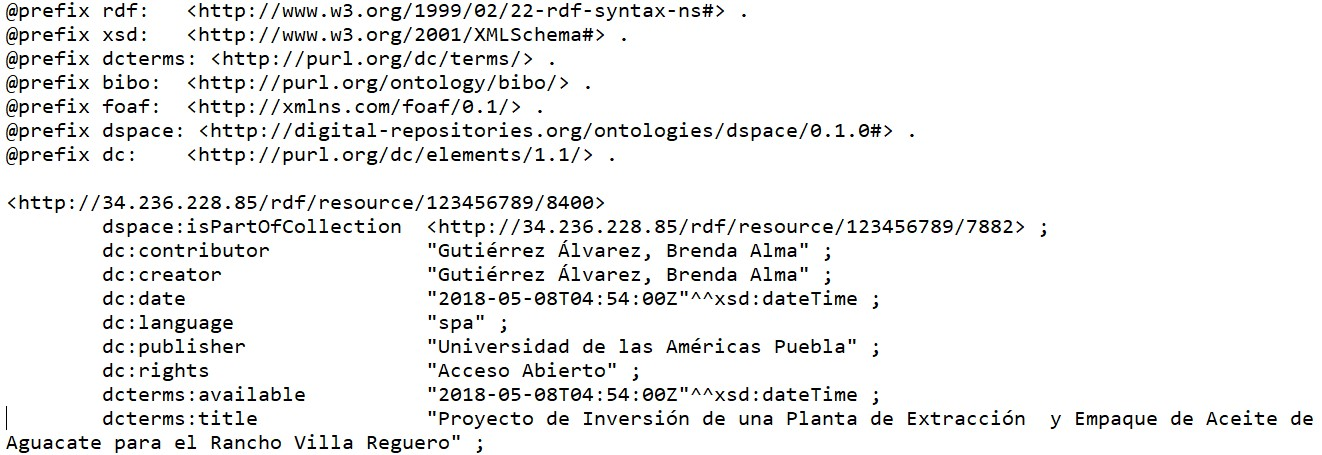
\includegraphics[width=14cm]{figures/ejemploRDF.jpg}} %NOMBRE DE LA FIGURA y TAMAÑO
    \caption{Ejemplo de conjunto de ternas en RDF} %PIE DE LA IMAGEN
    \label{ejemploRDFternas}
\end{figure}
  
    \part{Metodología} 
	\renewcommand{\chaptername}{Cap\'itulo}
\chapter{Metodolog\'ia}
\label{Metodologia}

El cap\'titulo \ref{Metodologia} se organiza como sigue: al inicio se presentan  los modelos empleados para el desarrollo del servicio web, despu\'es, se describe el \textit{an\'alisis de requerimientos} que determina las actividades clave. Posteriormente, en la etapa de \textit{dise\~{n}o} de explican los modelos de referencia y en la \textit{implementaci\'on} se trabajan con etapas. Finalmente, se presenta una herramienta de \textit{evaluaci\'on} para estimar la usabilidad del servicio y se enumeran las tareas de \textit{mantenimiento}.

\section{Modelo de desarrollo}

Para el desarrollo del servicio web se emplearon principalmente dos modelos en distintos momentos, como modelo base, se emplea el de cascada \cite{IngDeSW} para las etapas de an\'alisis de requerimientos y dise\~{n}o, para las etapas subsecuentes, se adapt\'o el modelo incremental como una etapa m\'as que consiste en la codificaci\'on de m\'odulos reducidos, pruebas r\'apidas de funcionamiento, realimentaci\'on, correcci\'on, liberaci\'on o escalamiento para llegar a la implementaci\'on; la etapa final es la de mantenimiento como muestra la Figura \ref{modeloDesarrolloSW}. La descripci\'on de este modelo de  desarrollo se presenta en las secciones posteriores. 

\begin{figure}[!ht]
	\centering
	\fbox{
	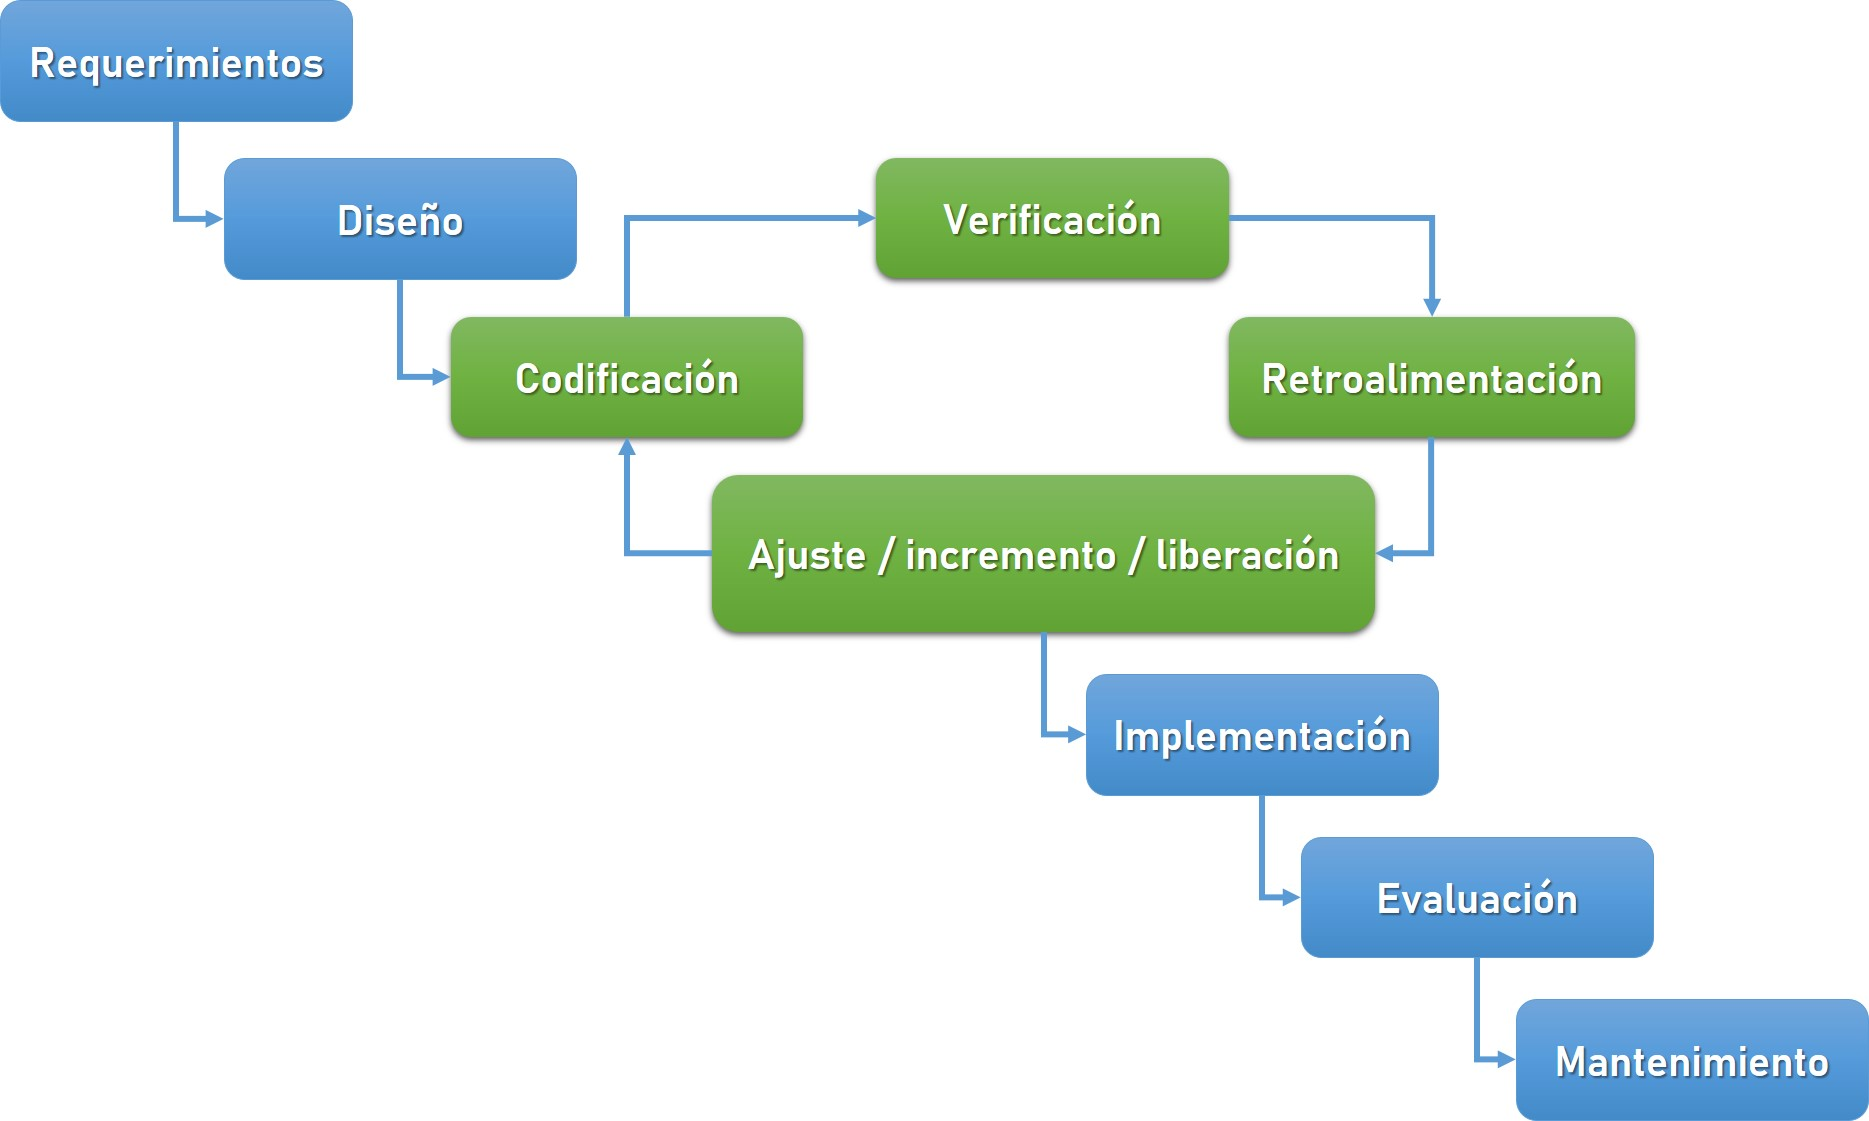
\includegraphics[width=12cm]{figures/ModeloDesarrolloSW.jpg}}
    \caption{Modelo de desarrollo del servicio web} %PIE DE LA IMAGEN
    \label{modeloDesarrolloSW}
\end{figure}

\section{An\'alisis de requerimientos}

El servicio web propuesto es parte del \emph{back end} del RI-UPPue,  el usuario final no tendr\'a una interacci\'on con \'este, sino que est\'a dise\~{n}ado para usuarios de tipo administrador. Junto con la administradora del RI-UPPue, se identificaron los requerimientos funcionales de la Tabla \ref{tablaRequerimientos}. 

\begin{table}[htbp]
    \begin{center}
    \caption{Tabla de requerimientos funcionales del servicio web}

    \begin{tabular}{|c|l|c|}
    \hline
    \centering \textbf{No. } & \textbf{Descripci\'on} & \textbf{Prioridad} \\
    \hline \hline
    1 & Consulta de informaci\'on sem\'antica & Alta  \\ \hline
    2 & Capacidad de almacenamiento de ternas en RDF & Alta  \\ \hline
    3 & Exportaci\'on de datos en formatos no propietarios como JSON y RDF & Mediana  \\ \hline
    4 & Integraci\'on de datos provenientes de otros RIs & Mediana  \\ \hline
    \end{tabular}
    \label{tablaRequerimientos}
    \end{center}
\end{table}

\section{Dise\~{n}o}

En la tesis se usan herramientas de modelado UML y los requerimientos planteados en la etapa de an\'alisis para elaborar los modelos de casos de uso, diagrama de clases y dise\~{n}o de alto nivel del servicio web, los cuales de describe a continuaci\'on.


\subsection{Casos de uso}

La Figura \ref{casoUso1} muestra el diagrama de casos de uso que modela la funcionalidad general del RI-UPPue.

\begin{figure}[!ht]
	\centering
	\fbox{
	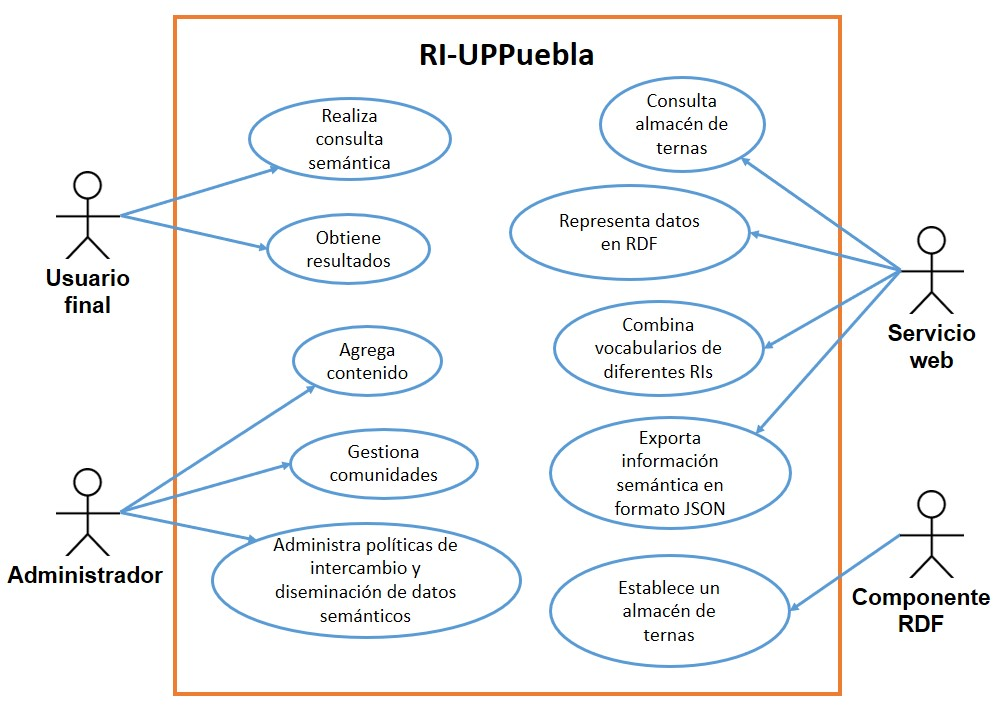
\includegraphics[width=12cm]{figures/CasoDeUso.jpg}} %NOMBRE DE LA FIGURA y TAMA\~{n}O
    \caption{Diagrama de casos de uso} %PIE DE LA IMAGEN
    \label{casoUso1}
\end{figure}

\subsection{Diagrama de clases}

La Figura \ref{diagramaClases1} muestra el diagrama de clases del servicio web, los rect\'angulos en color verde representan los nombres de las clases. Este dise\~{n}o se propuso en el art\'iculo \cite{SOMIdiseno}, en el cual se encuentra la descripci\'on detallada de los atributos y m\'etodos definidos para cada clase.

\begin{figure}[!ht]
	\centering
	\fbox{
	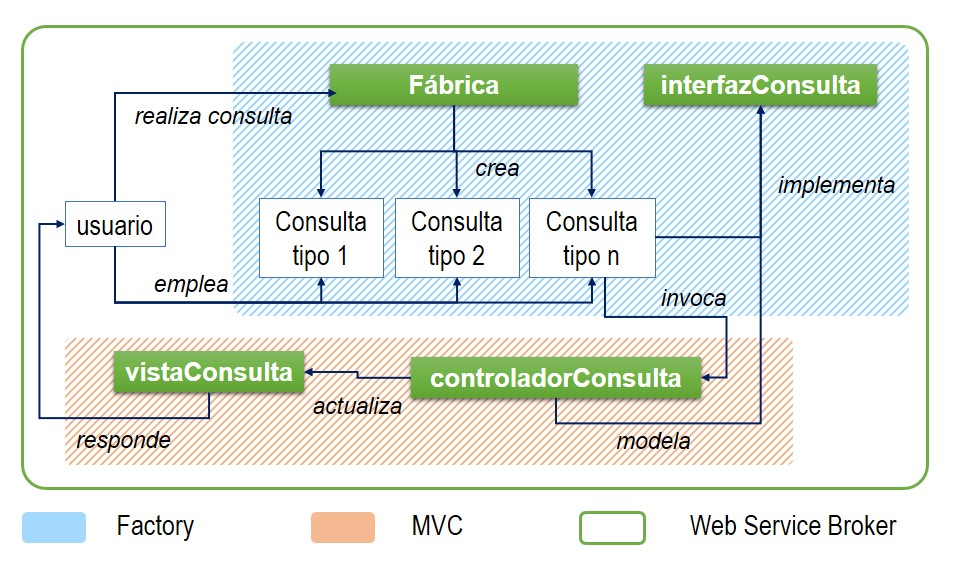
\includegraphics[width=12cm]{figures/Diagramadeclases1.jpg}} %NOMBRE DE LA FIGURA y TAMA\~{n}O
    \caption{Diagrama de clases. Fuente: \cite{SOMIdiseno}} %PIE DE LA IMAGEN
    \label{diagramaClases1}
\end{figure}

\subsection{Dise\~{n}o de alto nivel}

Las Figuras \ref{disenoAlto1} y \ref{disenoAlto2} muestran los dise\~{n}os elaborados para representar, por un lado, la manera en que se puede emplear el servicio web,  por otro lado, un modelo general del comportamiento en un contexto general, donde a corto plazo, se propone que opere en el  servidor del RI-UPPue y a mediano plazo, se buscar\'a su instalaci\'on en diferentes RIs que compartan la plataforma tecnol\'ogica DSpace.

\begin{figure}[!ht]
	\centering
	\fbox{
	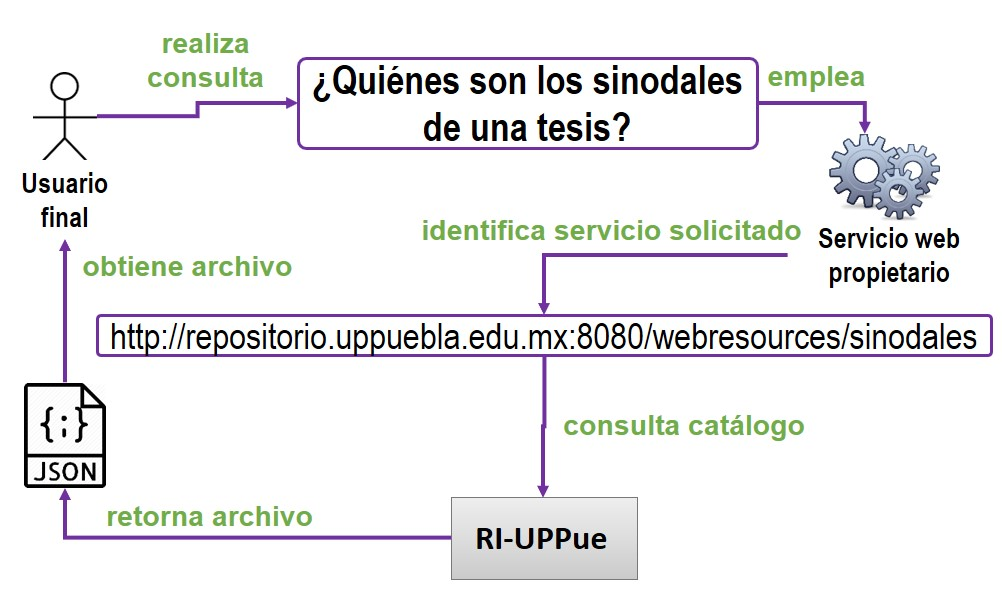
\includegraphics[width=12cm]{figures/DisenoAltoNivel1.jpg}} %NOMBRE DE LA FIGURA y TAMA\~{n}O
    \caption{Dise\~{n}o de consumo del servicio web. Fuente: \cite{SOMIdiseno}} %PIE DE LA IMAGEN
    \label{disenoAlto1}
\end{figure}

\begin{figure}[!ht]
	\centering
	\fbox{
	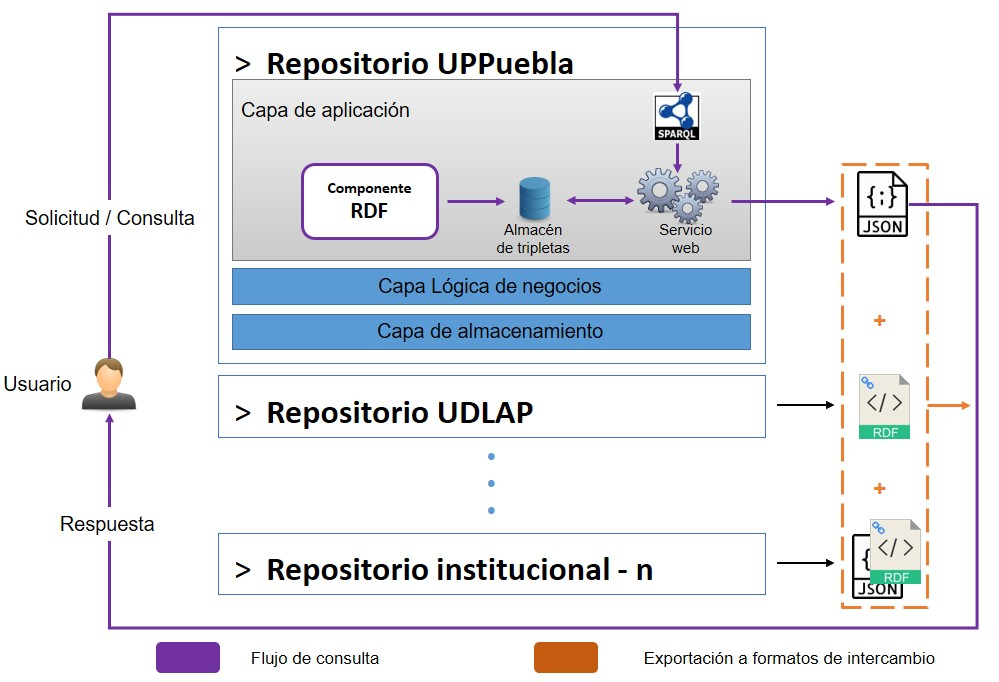
\includegraphics[width=12cm]{figures/DisenoAltoNivel2.jpg}} %NOMBRE DE LA FIGURA y TAMA\~{n}O
    \caption{Dise\~{n}o de alto nivel del servicio web. Fuente: \cite{SOMIdiseno}} %PIE DE LA IMAGEN
    \label{disenoAlto2}
\end{figure}

\section{Implementaci\'on}

Previo a la implementaci\'on de los m\'odulos, se asume que est\'a instalada la plataforma DSpace 6.2. Los pre-requisitos de operaci\'on para el servicio se relacionan con los elementos que muestra la Figura \ref{adicionalesDspace}, la cual contiene la arquitectura de la plataforma DSpace junto con los servicios adicionales que pueden ser habilitados. Cabe mencionar que la documentaci\'on de referencia de \cite{DSpaceRef} indica que DSpace cuenta con un m\'odulo RDF, sin embargo, \'este no se habilita durante la instalaci\'on est\'andar.

\begin{figure}[!ht]
	\centering
	\fbox{
	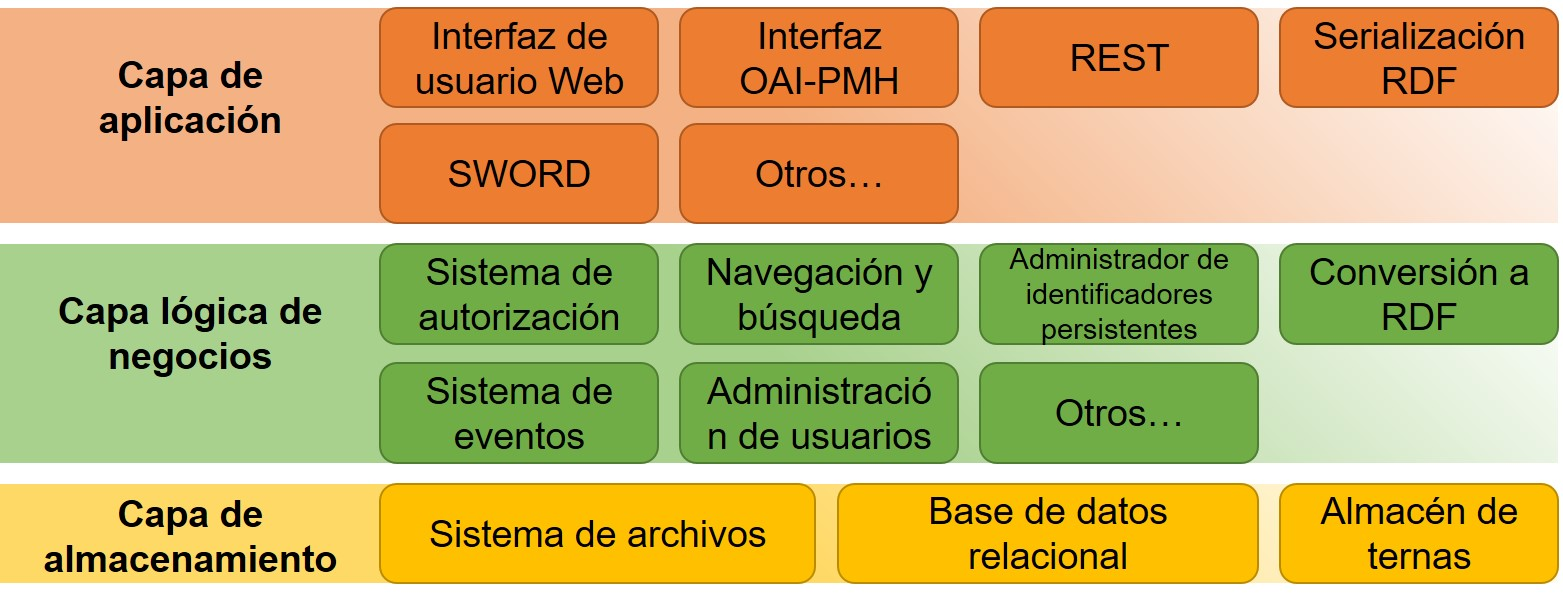
\includegraphics[width=12cm]{figures/ModulosAdicionalesDSpace62.jpg}} %NOMBRE DE LA FIGURA y TAMA\~{n}O
    \caption{M\'odulos adicionales de DSpace para la versi\'on 6.2} %PIE DE LA IMAGEN
    \label{adicionalesDspace}
\end{figure}

La habilitaci\'on del m\'odulo de serializaci\'on RDF requiere de tres elementos de software: 1) un almac\'en de ternas, 2) un mecanismo de serializaci\'on y 3) un conversor a formato RDF. La instalaci\'on de estos elementos forman parte de las etapas del proceso t\'ecnico que muestra la Figura \ref{etapasMigracion}, estas etapas se describen en las secciones siguientes.

\begin{figure}[!ht]
	\centering
	\fbox{
	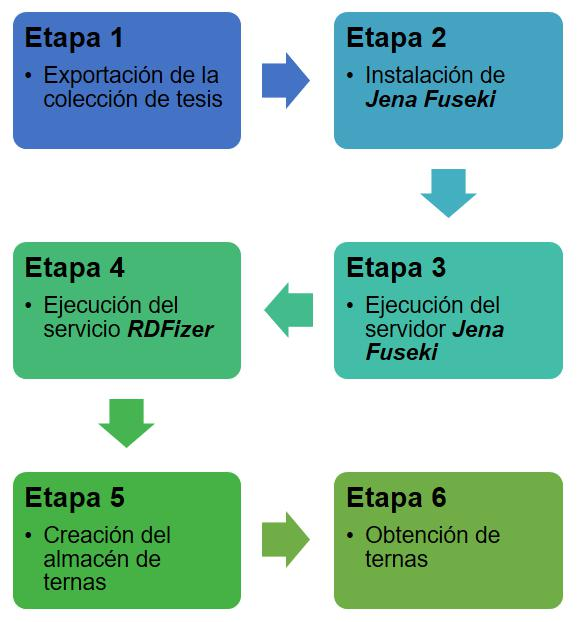
\includegraphics[width=10cm]{figures/etapasMigracion.jpg}} %NOMBRE DE LA FIGURA y TAMA\~{n}O
    \caption{Etapas del proceso de migraci\'on de metadatos del RI-UPPue a la web sem\'antica} %PIE DE LA IMAGEN
    \label{etapasMigracion}
\end{figure}

\subsection{Etapa 1: exportaci\'on de la colecci\'on de tesis}

DSpace permite exportar cualquier colecci\'on, en particular, se emplea la colecci\'on de tesis del RI-UPPue, formada por m\'as de  50 tesis del Departamento de Posgrado. La Figura \ref{exportacion-csv} muestra la interfaz para esta tarea, los metadatos se almacenan a un archivo con extensi\'on CSV\footnote{Siglas del ingl\'es de \emph{Comma Separated Values}, formato separado por comas}. El n\'umero 1 muestra el bot\'on para exportar y el 2 el archivo CSV con los metadatos exportados. La tarea de exportaci\'on se llev\'o a cabo al utilizar la versi\'on 75.0.3770.142 del navegador Chrome y la interfaz en JSP de DSpace.

\begin{figure}[!ht]
	\centering
	\fbox{
	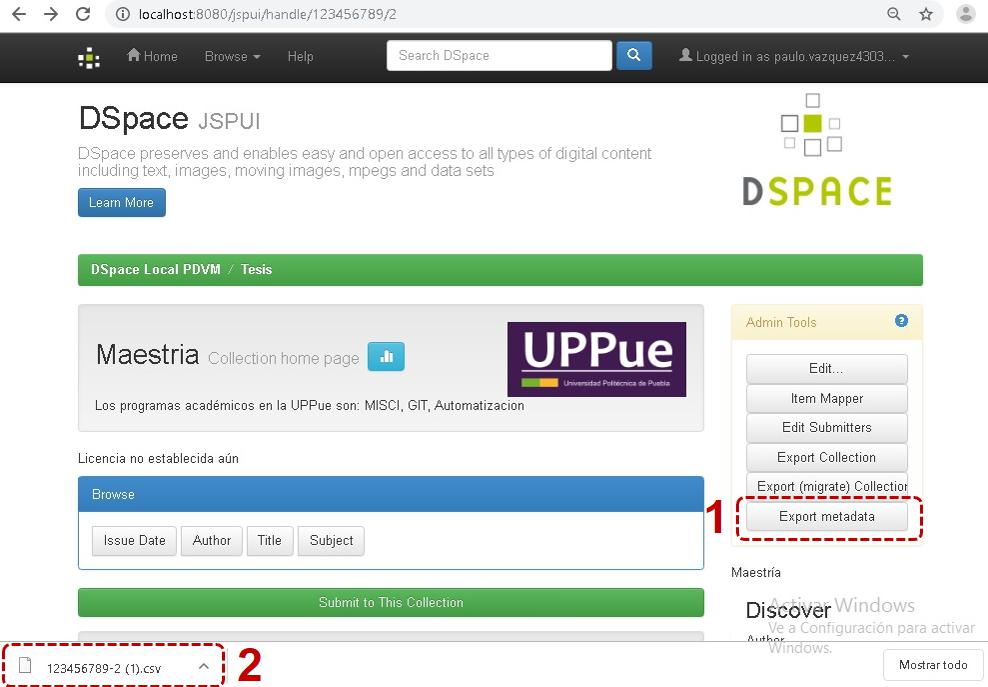
\includegraphics[width=12cm]{figures/exportarCSV.jpg}} 
    \caption{Exportaci\'on de la colecci\'on tesis a \textit{CSV}}
    \label{exportacion-csv}
\end{figure}

\subsection{Etapa 2: instalaci\'on de Apache Jena Fuseki}

El almac\'en de ternas es Jena-Fuseki versi\'on 1.6.0, este servidor provee tambi\'en de una interfaz web para realizar consultas en lenguaje SPARQL. Fuseki se integra con TDB\footnote{Componente de Jena Fuseki para el almacenamiento y consulta de datos en RDF} para proporcionar una capa de almacenamiento persistente transaccional y robusta, permite consultas de texto y consultas espaciales \cite{JenaFuseki}. La p\'agina oficial de Apache Jena Fuseki\footnote{Disponible en https://jena.apache.org/download/index.cgi} prove\'e diversas opciones para la descarga dependiendo del sistema operativo: Linux (.tar.gz) o Windows(.zip). 

\begin{figure}[!ht]
	\centering
	\fbox{
	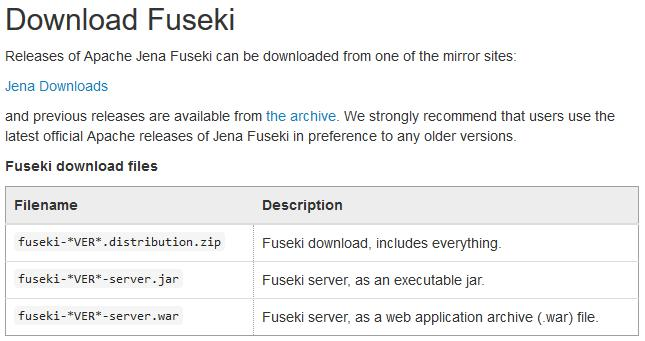
\includegraphics[width=12cm]{figures/opcionesDescargaFuseki.jpg}} 
    \caption{Opciones de descarga para el almac\'en de ternas Jena Fuseki}
\label{opcionesDescargaFuseki}
\end{figure}

Para terminar la instalaci\'on, los archivos descargados se descomprimen y se guardan en una carpeta que se nombra como \textit{Fuseki}. 

\begin{figure}[!ht]
	\centering
	\fbox{
	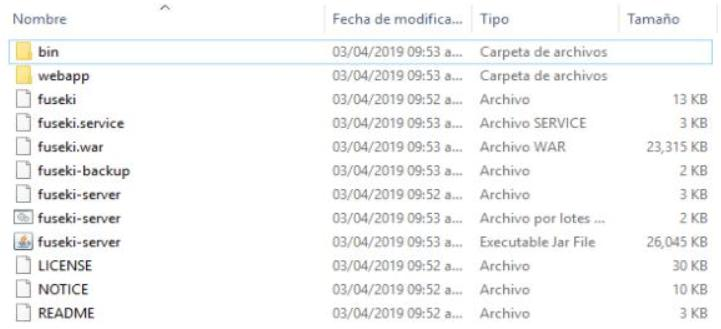
\includegraphics[width=12cm]{figures/contenidoCarpetaJena.jpg}} 
    \caption{Contenido de la carpeta del servidor \textit{Jena Fuseki}}
    \label{opcionesDescargaFuseki}
\end{figure}

\subsection{Etapa 3: ejecuci\'on del servidor Jena Fuseki}

Jena Fuseki se ejecuta como servicio de sistema operativo, como aplicaci\'on web Java (WAR) o como servidor independiente. El componente \texttt{Apache Shiro} se utiliza para implementar caracter\'isticas de seguridad, tiene una interfaz de usuario para el monitoreo y la administraci\'on. Jena Fuseki se inicializa ejecutando el archivo \textit{fuseki-server.bat}, (\textit{.jar} en Linux) como muestra la Figura \ref{ejecucionFuseki}.

\begin{figure}[!ht]
	\centering
	\fbox{
	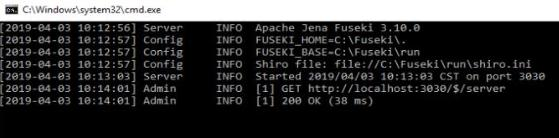
\includegraphics[width=12cm]{figures/ejecucionFuseki.jpg}} 
    \caption{Ejecuci\'on del servidor Jena Fuseki en terminal de Windows}
    \label{ejecucionFuseki}
\end{figure}

\subsection{Etapa 4: ejecuci\'on del servicio RDFizer}

Un componente \texttt{RDFizer} \cite{RDFizer} o \textit{spongers}, transforma datos de DSpace en una o m\'as de las serializaciones al modelo de datos RDF. La Figura \ref{etl-diagrama} representa esta transformaci\'on. Los \texttt{RDFizers} implementan  las tareas b\'asicas siguientes: extraer, transformar y cargar, en ingl\'es, \emph{extract}, \emph{transform} y \emph{load} (ETL), mismas que se describen como sigue: 

\begin{itemize}
    \item \textit{Extraer}. Los datos se obtienen de una base de datos o se recopilan de m\'ultiples y diversas fuentes 
    
    \item \textit{Transformar}. Los datos obtenidos se transforman en los requeridos mediante formularios; la transformaci\'on utiliza reglas o tablas de b\'usqueda o combina los datos con otros.
    
    \item \textit{Cargar}. Los datos se escriben en la fuente o base de datos destino. 
\end{itemize}

\begin{figure}[!ht]
	\centering
	\fbox{
	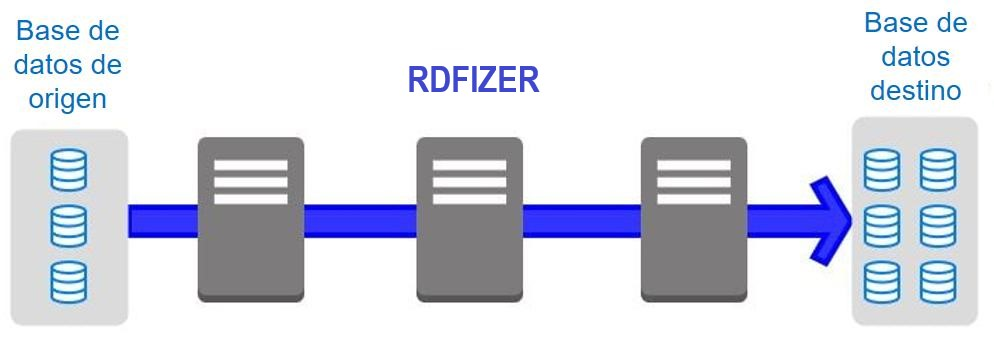
\includegraphics[width=12cm]{figures/etl.jpg}} 
    \caption{Extracci\'on, transformaci\'on y carga}
    \label{etl-diagrama}
\end{figure}

Los \texttt{RDFizers} soportan la migraci\'on de los metadatos a formatos de intercambio como XML, RDF o JSON. 

\subsection{Etapa 5: creaci\'on del almac\'en de ternas}

Una vez que los metadatos del repositorio se han procesado por los RDFizes o ETLs, los archivos con datos en RDF se almacenan en la ubicaci\'on indicada en el archivo de configuraci\'on de la plataforma DSpace \textit{fuseki-assembler-ttl}, forman as\'i el almac\'en de ternas o servicio persistente.

\subsection{Etapa 6: obtenci\'on de ternas}

Los metadatos en RDF para cada tesis se acceden empleando una direcci\'on de internet o URL\footnote{Localizador Uniforme de recursos, en ingl\'es \textit{Uniform Resource Locator}} como muestra la Figura \ref{accesoRdf}.\newline

\begin{figure}[!ht]
	\centering
	\fbox{
	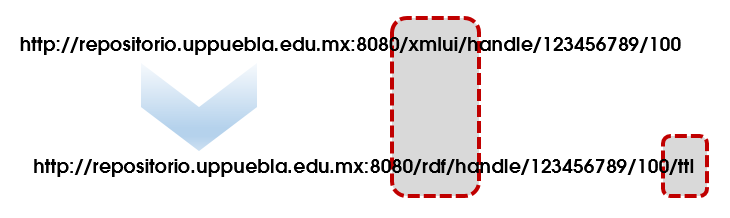
\includegraphics[width=12cm]{figures/xmluiRdf.png}} 
    \caption{Acceso a metadatos de tesis en RDF}
    \label{accesoRdf}
\end{figure}

La Figura \ref{resultadoRdf} muestra algunos metadatos de una tesis en RDF. Note que el archivo RDF contiene los metadatos capturados en la plataforma DSpace cuando se agrega un documento a la colecci\'on. En el ejemplo, se muestra un error l\'ogico, notar que los elementos \texttt{creator} y \texttt{contributor} contienen el mismo valor.

\begin{figure}[!ht]
	\centering
	\fbox{
	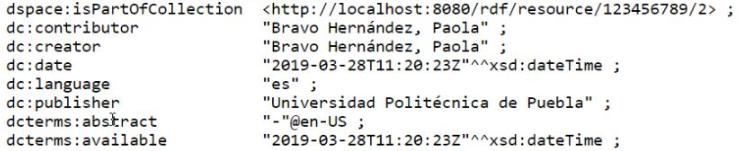
\includegraphics[width=12cm]{figures/extractoMetadatosRDF.jpg}} 
    \caption{Metadatos de RDF para una tesis del almac\'en de ternas}
    \label{resultadoRdf}
\end{figure}

\subsection{Interfaz gr\'afica de usuario}

La interfaz gr\'afica de usuario (\emph{Graphical User Interface}, GUI) o \emph{front end} del servicio web propuesto, integra tres tecnolog\'ias web: 
\emph{HTML 5}, lenguaje de modelado de hipertexto, en ingl\'es \emph{HiperText Markup Language}, que es un lenguaje de marcado que sirve para modelar contenidos; \emph{Java Script}, que es un lenguaje de programaci\'on del lado del cliente para manipular elementos HTML y hojas de estilo en cascada, en ingl\'es \emph{Cascading Style Sheets} (CSS), que sirven para definir reglas de dise\~{n}o para la presentaci\'on del contenido. Estas tecnolog\'ias son nativas a la web por lo que no se requiere de ning\'un tipo de instalaci\'on adicional, ya que ejecuci\'on de los modelos se realiza a trav\'es del uso navegadores como  Chrome, Mozilla, Opera, Edge o Safari.

\subsection{Herramientas software}

Esta secci\'on contiene una breve descripci\'on de las herramientas de software utilizadas en la implementaci\'on del servicio web. 

\subsubsection{Servicio especializado en lenguaje Python 3.6}

Se utiliz\'o la versi\'on 3.6 del lenguaje de programaci\'on Python para extraer elementos (\emph{\'items}) del almac\'en de ternas a trav\'es de la librer\'ia RDFLib  versi\'on 4.2.2  \cite{RDFlib} y as\'i integrar los datos provenientes del RI-UPPue a una instancia de la ontolog\'ia Onto4-RI-UPPue a trav\'es de la librer\'ia OWLReady2 \cite{OWLReady2} versi\'on 0.19. La Figura \ref{arquitecturaServicio} muestra la arquitectura propuesta para el servicio web y sus componentes. 

\begin{figure}[!ht]
	\centering
	\fbox{
	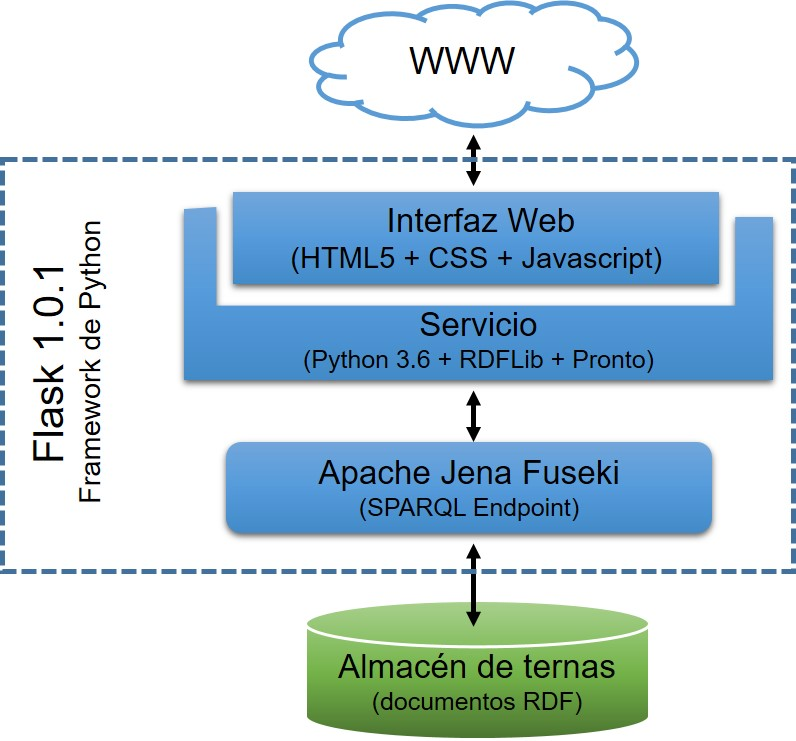
\includegraphics[width=10cm]{figures/ArquitecturaSW.jpg}} 
    \caption{Arquitectura del servicio web}
    \label{arquitecturaServicio}
\end{figure}

La Figura \ref{tecnologiasServicio} muestra las tecnolog\'ias empleadas para el desarrollo del servicio web desde el punto de vista del \emph{front end} (parte gr\'afica del servicio web) y del \emph{back end} (parte l\'ogica del servicio web).

\begin{figure}[!ht]
	\centering
	\fbox{
	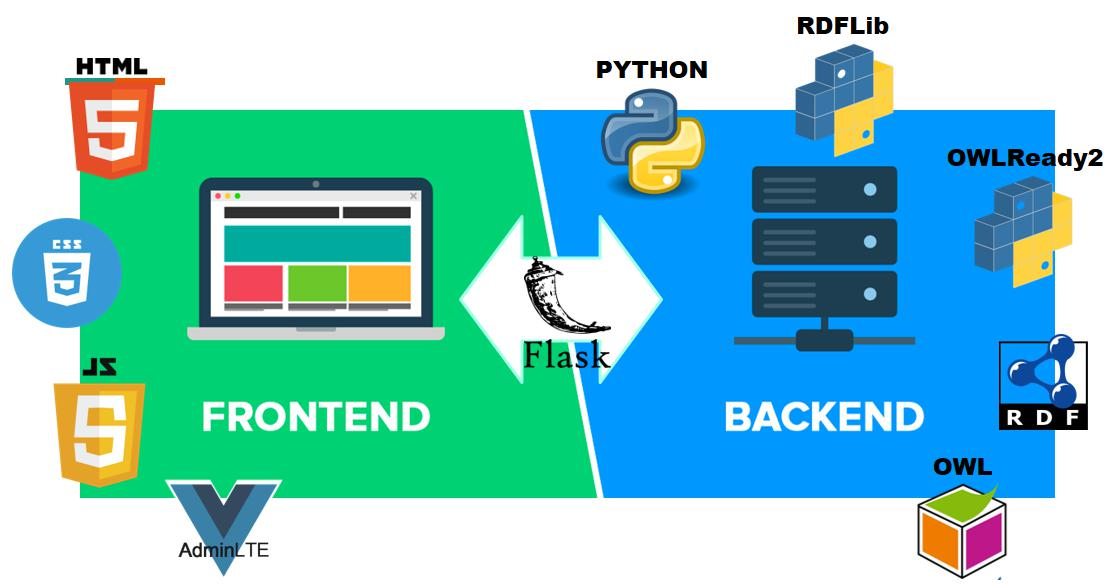
\includegraphics[width=12cm]{figures/tecnologiasServicoWeb.jpg}} 
    \caption{Tecnolog\'ias empleadas en el servicio web}
    \label{tecnologiasServicio}
\end{figure}

\subsubsection{Librer\'ia RDFLib}

La librer\'ia \texttt{RDFLib}\footnote{Disponible en: \textit{https://pypi.org/project/rdflib/}} de Python sirve para trabajar con datos en RDFen diferentes sintaxis como \texttt{RDF/XML, N3, NTriples, Turtle, TriX, RDFa} y \texttt{Microdata}; su interfaz \textit{Graph} puede ser respaldada por cualquiera de las implementaciones de \textit{Store}. El n\'ucleo \texttt{rdflib} incluye implementaciones de \texttt{Store} para almacenamiento en memoria, almacenamiento persistente (en Berkeley DB) y un contenedor para puntos finales remotos de SPARQL, incluye el motor de consulta SPARQL 1.1.

La instalaci\'on de \texttt{RDFLib} se realiza a trav\'es del servicio \textit{pip}\footnote{Repositorio de software para el lenguaje Python, en ingl\'es \textit{Python Index Package} } de Python mediante la instrucci\'on \texttt{pip install rdflib} como se indica en la documentaci\'on de este lenguaje. 

\subsubsection{Librer\'ia OWLReady2}

La librer\'ia OWLReady2\footnote{Disponible en \emph{https://pypi.org/project/Owlready2/}}  de Python se usa trabajar con ontolog\'ias escritas en la versi\'on 2.0 de OWL, las cuales se gestionan como objetos Python. La librer\'ia soporta la conexi\'on el razonador Hermit y tareas como las siguientes: 

\begin{itemize}
    \item Importaci\'on de ontolog\'ias OWL 2.0 en NTriples, RDF/XML o formato OWL/XML.
    \item Exportaci\'on de ontolog\'ias OWL 2.0 a NTriples o RDF/XML
    \item Manipulaci\'on de clases, instancias y propiedades de las ontolog\'ias de forma transparente, como si fueran objetos de Python
    \item Agregaci\'on de m\'etodos de Python a las clases de una ontolog\'ia
    \item Clasificaci\'on autom\'atica de clases e instancias utilizando los razonadores HermiT o Pellet 
    \item Compatibilidad con la librer\'ia RDFlib 
  \end{itemize}

\subsubsection{Librer\'ia xml.etree.ElementTree}

La librer\'ia \textit{xml.etree.ElementTree}\footnote{Disponible en \textit{https://pypi.org/project/elementtree/}} se usa para procesar documentos XML, cuenta con diversos m\'etodos para acceder a elementos espec\'ificos de un documento, insertar, modificar y eliminar nodos. En la tesis, esta librer\'ia se utiliza para obtener informaci\'on de la ontolog\'ia Onto4RI-UPPue escrita en OWL.

\subsubsection{Framework Flask}

El desarrollo del servicio web emplea la versi\'on 1.1.1 de Flask \footnote{Disponible en \emph{https://pypi.org/project/Flask/}}, el cual es un \emph{framework} ligero para aplicaciones web, es decir, entorno de trabajo o marco de trabajo, conjunto estandarizado de conceptos, pr\'acticas y criterios para enfocar un tipo de problem\'atica particular que sirve como referencia para enfrentar y resolver nuevos problemas de \'indole similar. 

Flask est\'a dise\~{n}ado para desarrollar proyectos de manera r\'apida y relativamente sencilla con capacidad para escalar a aplicaciones complejas, implementa el patr\'on de dise\~{n}o Modelo-Vista-Controlador (MVC), en ingl\'es \emph{Model-View-Controller}, ampliamente usado en el desarrollo de proyectos de software. 

\subsubsection{AdminLTE}
Finalmente, en el desarrollo del \emph{front end} se integra el panel de control o \emph{Dashboard} que conforma un tipo de interfaz gr\'afica de usuario con\emph{AdminLTE},  versi\'on 2.4.15.

\section{Evaluaci\'on}

Las pruebas de usabilidad orientadas a la experiencia del usuario \footnote{Tambi\'en conocido como \emph{UX}, en ingl\'es \emph{User eXperience}} se basan en la observaci\'on y an\'alisis de un grupo de usuarios reales empleando el servicio web, con objeto de identificar los problemas de uso. El servicio web se eval\'ua a trav\'es de una adaptaci\'on de la plantilla para hacer an\'alisis heur\'isticos de usabilidad\footnote{Disponible en \emph{https://www.torresburriel.com/weblog/2008/11/28/plantilla-para-hacer-analisis-heuristicos-de-usabilidad/}} propuesta por \cite{OnceHeuristicas}. La herramienta consta de un cuestionario que explora once heur\'isticas y en donde el evaluador (en este caso, un usuario) indica seg\'un una escala de Likert de cinco grados, su grado de satisfacci\'on. La Tabla \ref{tablaEscalasLikert} muestra las escalas con las que se eval\'uan cada una de las heur\'isticas.\newline

\begin{table}[htbp]
    \begin{center}
    \caption{Escala de Likert empleada para evaluar el servicio web}
    \begin{tabular}{| p{1.5cm}| p{11cm} |}
    \hline
    \centering \textbf{Valor } & \textbf{Observaciones} \\
    \hline \hline
    1 & Se da la m\'inima expresi\'on del heur\'istico en las p\'aginas evaluadas \\ \hline
    2 & Se da una expresi\'on baja del heur\'istico en las p\'aginas evaluadas \\ \hline
    3 & Se da una expresi\'on media del heur\'istico en las p\'aginas evaluadas \\ \hline
    4 & Se da una expresi\'on alta del heur\'istico en las p\'aginas evaluadas \\ \hline
    5 & Se da la m\'axima expresi\'on del heur\'istico en las p\'aginas evaluadas \\ \hline
    \end{tabular}
    \label{tablaEscalasLikert}
    \end{center}
\end{table}

Las heur\'isticas evaluadas son las siguientes:

\begin{itemize}
    \item Generalidades
    \item Identidad e informaci\'on
    \item Lenguaje y redacci\'on
    \item Rotulado
    \item Estructura y navegaci\'on
    \item Estructura de la p\'agina
    \item B\'usqueda
    \item Elementos multimedia
    \item Ayuda
    \item Accesibilidad
    \item Control y retroalimentaci\'on
\end{itemize}

\begin{figure}[!ht]
	\centering
	\fbox{
	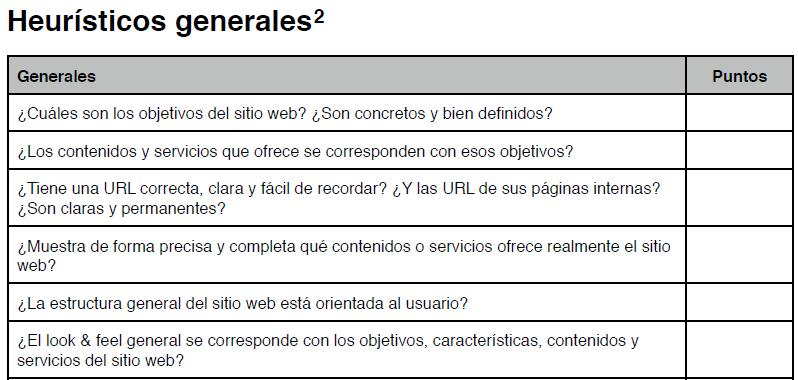
\includegraphics[width=12cm]{figures/extractoPlantilla.jpg}} 
    \caption{Extracto de la plantilla para hacer an\'alisis heur\'isticos de usabilidad}
    \label{extractoPlantilla}
\end{figure}

\section{Mantenimiento}

La fase final del desarrollo del servicio web consta de realizar las modificaciones o adecuaciones identificadas en la etapa de evaluaci\'on.

    \part{Resultados} 
	\renewcommand{\chaptername}{Capitulo}
\chapter{Resultados} 
\section{Resultados}

Conforme a la metodolog\'ia planteada para el desarrollo del servicio web, la figura \ref{esquemaResultados} muestra cada proceso o tarea efectuada, donde los resultados obtenidos en cada una de las fases completadas son descritos en \'este cap\'itulo.

\begin{figure}[!ht]
	\centering
	\fbox{
	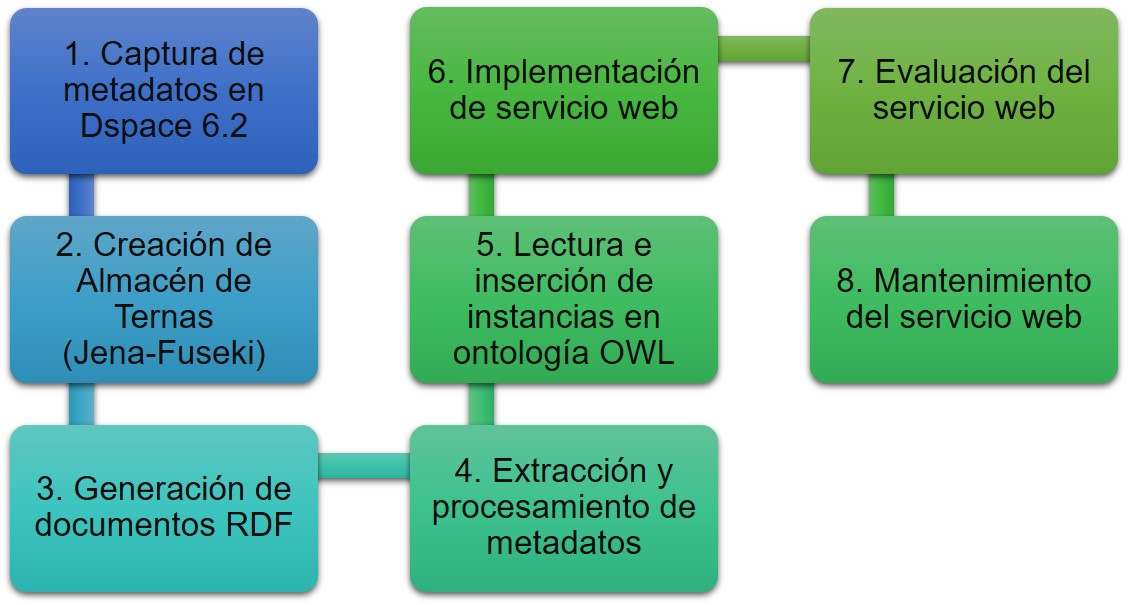
\includegraphics[width=12cm]{figures/etapaResultados.jpg}} 
    \caption{Esquema general de fases para la obtenci\'on de resultados}
    \label{esquemaResultados}
\end{figure}

Adem\'as, se valid\'o el funcionamiento de los servicios tecnol\'ogicos tanto instalados, configurados o desarrollados, a trav\'es de la verificaci\'on de los datos exportados e importados durante los siguientes procesos:

\begin{itemize}
    \item Exportaci\'on de metadatos en formato CSV
    \item Recuperaci\'on de metadatos del almac\'en de ternas en formato RDF
    \item Exportaci\'on de datos a formato JSON
    \item Integraci\'on de instancias a la ontolog\'ia Onto4RI-UPPue en formato OWL
    \item Verificaci\'on del funcionamiento de la interfaz web
\end{itemize}

\subsection{Fase 1. Captura de metadatos en DSpace 6.2}

Dentro de esta etapa se realizaron las siguientes actividades:

\begin{itemize}
    \item Instalaci\'on de una instancia local de la plataforma DSpace versi\'on 6.2, para la realizaci\'on de pruebas emulando las mismas condiciones t\'ecnicas del RI-UPPue
    \item Creaci\'on de una comunidad \textit{Tesis}, Figura \ref{creacionComunidad}
    \item Creaci\'on de la colecci\'on \textit{Maestr\'ia}, Figura \ref{creacionColeccion}
    \item Inserci\'on de once \'items: \textit{metadatos + archivos}, Figura \ref{itemsAgregados}
\end{itemize}{}

\begin{figure}[!ht]
	\centering
	\fbox{
	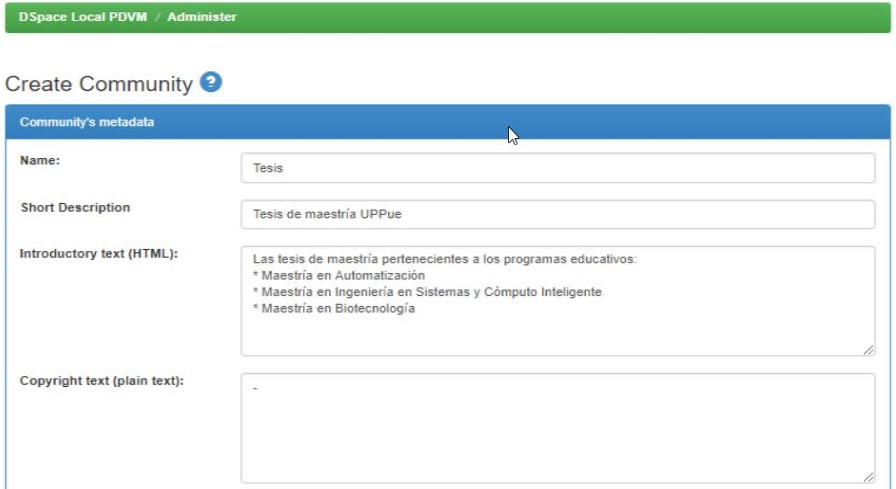
\includegraphics[width=12cm]{figures/creacionComunidad.jpg}} 
    \caption{Creaci\'on de la comunidad de \textit{tesis}}
    \label{creacionComunidad}
\end{figure}

\begin{figure}[!ht]
	\centering
	\fbox{
	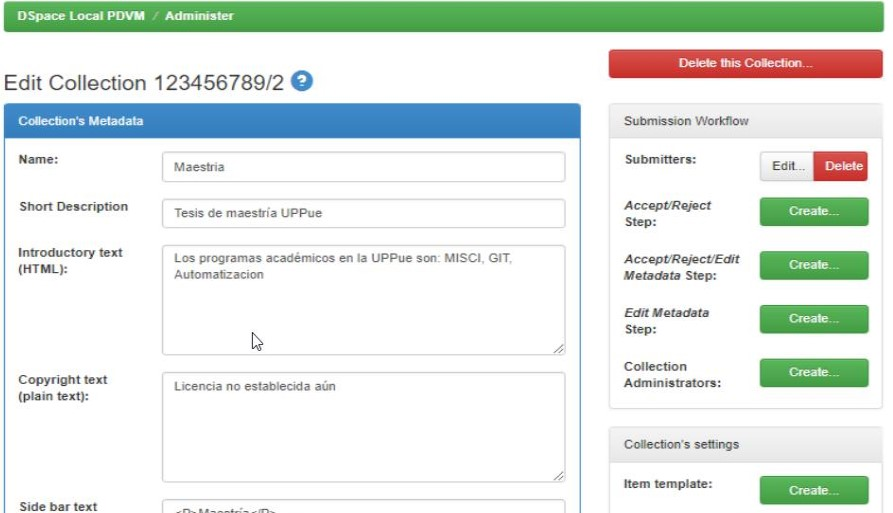
\includegraphics[width=12cm]{figures/creacionColeccion.jpg}} 
    \caption{Creaci\'on de la colecci\'on \textit{maestr\'ia}}
    \label{creacionColeccion}
\end{figure}

\begin{figure}[!ht]
	\centering
	\fbox{
	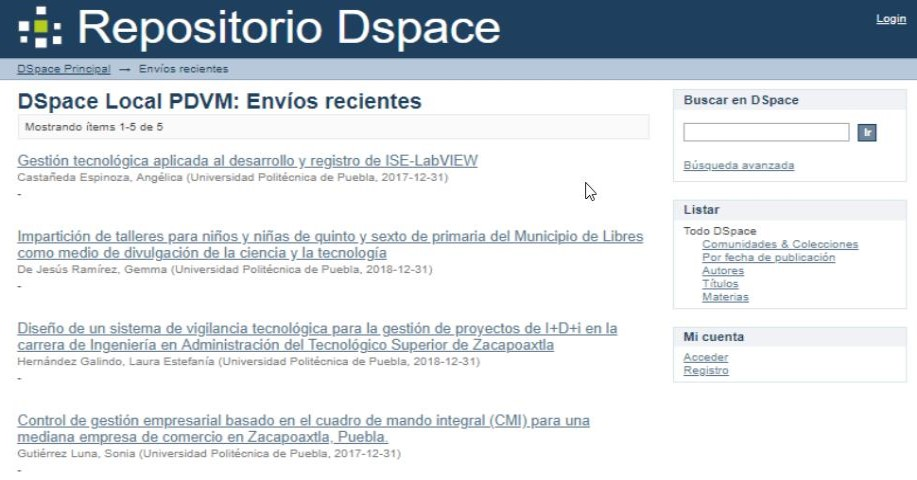
\includegraphics[width=12cm]{figures/itemsAgregados.jpg}} 
    \caption{\'items agregados a la comunidad de \textit{tesis}}
    \label{itemsAgregados}
\end{figure}

\subsection{Fase 2. Creaci\'on de almac\'en de ternas}

Se llev\'o a cabo la instalaci\'on del almac\'en de ternas conforme a las actividades descritas en la Figura \ref{instalacionTriplestore} para la instalaci\'on de los componentes necesarios para habilitar \'este servicio de tipo persistente.

\begin{figure}[!ht]
	\centering
	\fbox{
	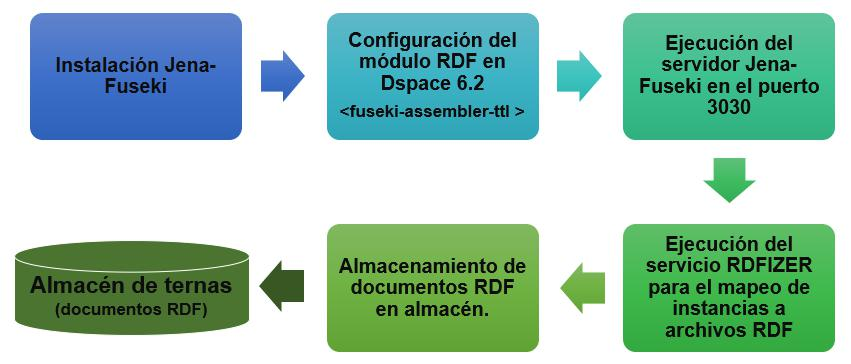
\includegraphics[width=12cm]{figures/InstalacionTripleStore.jpg}} 
    \caption{Implementaci\'on del almac\'en de ternas empleando el servidor Apache Jena Fuseki versi\'on 1.6}
    \label{instalacionTriplestore}
\end{figure}

El \textit{Anexo A} contiene un manual que describe de manera detallada la habilitaci\'on del componente RDF de la plataforma DSpace versi\'on 6.2 a trav\'es de la instalaci\'on del servidor Apache Jena Fuseki versi\'on 1.6, cuya ejecuci\'on se muestra en la Figura \ref{jenaFusekiCorriendo}, lo cual confirma su funcionamiento correcto.

\begin{figure}[!ht]
	\centering
	\fbox{
	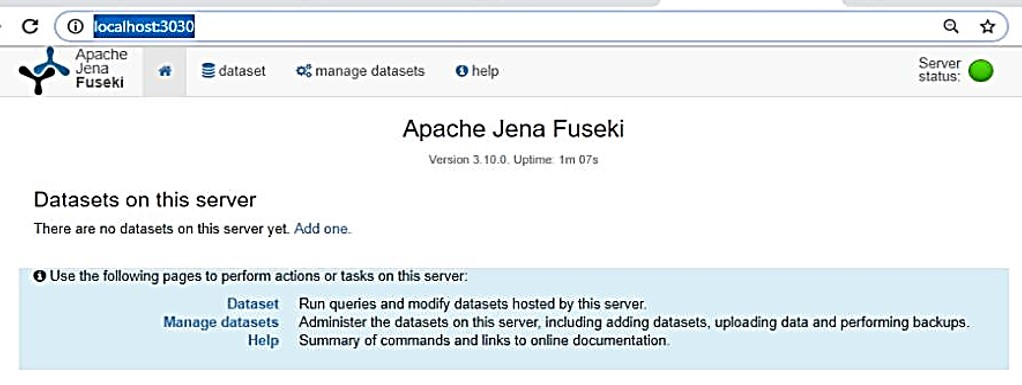
\includegraphics[width=12cm]{figures/ejecuccionJenaFuseki.jpg}} 
    \caption{P\'agina principal del servidor Apache Jena Fuseki corriendo en el servidor local}
    \label{jenaFusekiCorriendo}
\end{figure}

\subsection{Fase 3. Generaci\'on de documentos en RDF}

En esta fase, se realiz\'o la ejecuci\'on del serializador \textit{RDFizer} como se muestra en la Figura \ref{ejecucionRdfizer} para la extracci\'on de metadatos almacenados en DSpace y su migraci\'on al almac\'en de ternas.

\begin{figure}[!ht]
	\centering
	\fbox{
	\includegraphics[width=12cm]{figures/ejecucionRDFizer.jpg}} 
    \caption{Ejecuci\'on del serializador \textit{RDFizer}}
    \label{ejecucionRdfizer}
\end{figure}

Para la verificaci\'on de la migraci\'on de \'items almacenados en DSpace al almac\'en de ternas se realiz\'o la verificaci\'on de cada  documento RDF generado, en un conjunto experimental de once instancias agregadas previamente a la plataforma DSpace (ver la Tabla \ref{tablaInstanciasRdf}).

\begin{table}[htbp]
    \begin{center}
    \caption{Actividades de verificaci\'on con instancias migradas a almac\'en de ternas}
    \begin{tabular}{| p{1.5cm}| p{3.5cm} | p{3.5cm} | p{3.5cm} |}
    \hline
    \centering \textbf{No. } & \textbf{Actividad} & \textbf{Resultado esperado} & \textbf{Resultado obtenido} \\
    \hline \hline
    1 & Serializaci\'on de \'items almacenados en DSpace & Once instancias migradas a formato RDF & Once instancias migradas a formato RDF \\ \hline
    2 & Acceso a documento RDF mediante URL & Consulta de once documentos RDF & Consulta de once documentos RDF  \\ \hline
    \end{tabular}
    \label{tablaInstanciasRdf}
    \end{center}
\end{table}

\subsection{Fase 4. Extracci\'on y procesamiento de metadatos}

Se implement\'o un servicio (ver Figura \ref{claseExtraccion}) utilizando la versi\'on 3.6 del lenguaje Python y la librer\'ia RDFlib\footnote{Biblioteca de Python textitleada para trabajar con archivos XLM y RDF} para verificar autom\'aticamente el n\'umero de documentos migrados. La Tabla \ref{casosPruebaMetadatos} muestra los resultados. La figura \ref{metadatosRecuperados} muestra el resultado de ejecutar esta aplicaci\'on.\newline

\begin{table}[htbp]
    \begin{center}
    \caption{Actividades de verificaci\'on con archivos en RDF}
    \begin{tabular}{| p{1.5cm}| p{3.5cm} | p{3.5cm} | p{3.5cm} |}
    \hline
    \centering \textbf{No. } & \textbf{Acci\'on} & \textbf{Resultado esperado} & \textbf{Resultado obtenido} \\
    \hline \hline
    1 & Recuperaci\'on de archivos RDF integrados en el almac\'en de ternas  & Extracci\'on de once tesis & Extracci\'on de once tesis \\ \hline
    2 & Recuperaci\'on de los metadatos de un archivo RDF  & Recuperaci\'on de quince metadatos DCMI & Recuperaci\'on de doce metadatos DCMI, dos metadatos propios de DSpace y tres m\'as \\ \hline
    \end{tabular}
    \label{casosPruebaMetadatos}
    \end{center}
\end{table}

\begin{figure}[!ht]
	\centering
	\fbox{
	\includegraphics[width=12cm]{figures/claseExtraccion.jpg}} 
    \caption{Descripci\'on de la clase para la extracci\'on de metadatos desde archivo RDF}
    \label{claseExtraccion}
\end{figure}

La Figura \ref{metadatosRecuperados} muestra los metadatos migrados en formato RDF para una tesis.

\begin{figure}[!ht]
	\centering
	\fbox{
	\includegraphics[width=12cm]{figures/metadatosRecuperados.jpg}} 
    \caption{Metadatos recuperados para una instancia del almac\'en de ternas}
    \label{metadatosRecuperados}
\end{figure}

Para verificar los resultados del proceso de migraci\'on, se llev\'o a cabo la revisi\'on de los datos exportados al formato CSV y RDF a un conjunto de prueba experimental (ver la Tabla \ref{casosPruebaInstancias}).\newline

\begin{table}[htbp]
    \begin{center}
    \caption{Actividades de verificaci\'on con archivos CSV}
    \begin{tabular}{| p{1.5cm}| p{3.5cm} | p{3.5cm} | p{3.5cm} |}
    \hline
    \centering \textbf{No. } & \textbf{Actividad} & \textbf{Resultado esperado} & \textbf{Resultado obtenido} \\
    \hline \hline
    1 & Exportaci\'on de instancias en formato CSV & Archivo con once instancias & Archivo con once instancias  \\ \hline
    2 & Exportaci\'on de metadatos en formato CSV  & Archivo con quince metadatos DCMI & Archivo con dieciseis metadatos DCMI y dos metadatos DSpace \\ \hline
    \end{tabular}
    \label{casosPruebaInstancias}
    \end{center}
\end{table}

Los metadatos exportados en CSV son: \textit{id, collection, author, accessioned, available, issued, abstract, provenance, sponsorship, description, citation, uri, iso, publisher, subject, alternative title, title} y \textit{type}.\newline

\subsection{Fase 5. Lectura e inserci\'on de instancias en Onto4RI-UPPue}

El m\'etodo \textit{getroot} permite ubicarse en el nodo ra\'iz de \'arbol, y los m\'etodos \textit{set} y \textit{dump} se emplean para la inserci\'on de nuevos nodos en el cuerpo del documentos, conservando la estructura de las instancias ya existentes en la ontolog\'ia. La Figura \ref{insercionInstancias} muestra un extracto de la implementaci\'on de la inserci\'on de una instancia en la ontolog\'ia.

\begin{figure}[!ht]
	\centering
	\fbox{
	\includegraphics[width=12cm]{figures/insercionInstancia.jpg}} 
    \caption{M\'etodo de inserci\'on de instancias}
    \label{insercionInstancias}
\end{figure}

La Figura \ref{estructuraInstancia} muestra la estructura que deben guardar las instancias agregadas a la ontolog\'ia Onto4RI-UPPue mediante el servicio de integraci\'on.

\begin{figure}[!ht]
	\centering
	\fbox{
	\includegraphics[width=12cm]{figures/instanciaOntologia.jpg}} 
    \caption{Estructura de una instancia agregada por el servicio}
    \label{estructuraInstancia}
\end{figure}

\subsection{Fase 6. Implementaci\'on del servicio web}

La figura \ref{tecnologiasServicio} muestra las tecnolog\'ias empleadas para el desarrollo del servicio web, con lo que el servicio cuenta con las siguientes caracter\'isticas generales:

\begin{itemize}
    \item Responsividad
    \item Validaci\'on HTML
    \item Dinamismo
    \item Accesibilidad
    \item Intuitividad
\end{itemize}{}

El servicio web cuenta con las siguientes secciones:

\begin{itemize}
    \item Inicio
    \item B\'usqueda sem\'antica
    \item Test UX
    \item Exportar
    \item Preguntas frecuentes
    \item Contactos
\end{itemize}{}

Las figuras de la \ref{paginaInicial} a la \ref{paginaContactos} ilustran las secciones contenidas en el servicio web.\newline

La \textbf{p\'agina inicial} muestra un mensaje de bienvenida breve y un listado de los servicios ofrecidos por el servicio.\newline

\begin{figure}[!ht]
	\centering
	\fbox{
	\includegraphics[width=12cm]{figures/paginaInicial.jpg}} 
    \caption{P\'agina inicial del servicio web}
    \label{paginaInicial}
\end{figure}

El servicio de \textbf{b\'usqueda sem\'antica} muestra un panel para realizar b\'usquedas a trav\'es de criterios como \textbf{es autor} y \textbf{es sinodal} que establecen una relaci\'on entre las personas que participaron en la elaboraci\'on de una tesis de maestr\'ia.\newline

\begin{figure}[!ht]
	\centering
	\fbox{
	\includegraphics[width=12cm]{figures/paginaBusqueda.jpg}} 
    \caption{Servicio de b\'usqueda sem\'antica}
    \label{paginaSemantica}
\end{figure}

Una vez establecidos los criterios de b\'usqueda y el usuario da click en el bot\'on \textbf{Buscar} en la parte inferior del panel se listan los resultados en forma de tabla.\newline

\begin{figure}[!ht]
	\centering
	\fbox{
	\includegraphics[width=12cm]{figures/paginaResultados.jpg}} 
    \caption{Resultados de la de b\'usqueda sem\'antica}
    \label{paginaResultados}
\end{figure}

El servicio tambi\'en brinda la posibilidad de descargar la ontolog\'ia en dos formatos de intercambio de informaci\'on como lo son \textit{JSON} y \textit{OWL}, que son parseables por cualquier lenguaje de programaci\'on de alto nivel.\newline

\begin{figure}[!ht]
	\centering
	\fbox{
	\includegraphics[width=12cm]{figures/paginaExportar.jpg}} 
    \caption{Servicio para la descarga de la ontolog\'ia en formato JSON/OWL}
    \label{paginaExportar}
\end{figure}

De igual manera, se ofrece hay una secci\'on de preguntas frecuentes que el usuario del servicio web puede consultar para conocer m\'as a cerca de los conceptos b\'asicos y terminolog\'ia con la que no se encuentra familizarizado.\newline

\begin{figure}[!ht]
	\centering
	\fbox{
	\includegraphics[width=12cm]{figures/paginaPreguntas.jpg}} 
    \caption{P\'agina de preguntas frecuentes}
    \label{paginaPreguntas}
\end{figure}

Finalmente, se anexa una p\'agina con los datos de contactos tanto de la directora de proyecto, como del desarrollador del mismo.\newline

\begin{figure}[!ht]
	\centering
	\fbox{
	\includegraphics[width=12cm]{figures/paginaContactos.jpg}} 
    \caption{P\'agina de contactos}
    \label{paginaContactos}
\end{figure}

Adem\'as, el servicio web es accesible tanto en equipos de c\'omputo de escritorio y cualquier dispositivo m\'ovil que cuente con conexi\'on a Internet, y para cualquier tipo de sistema operativo, como lo muestra la Figura \ref{vistaMovil}.\newline

\begin{figure}[!ht]
	\centering
	\fbox{
	\includegraphics[width=12cm]{figures/vistaResponsiva.jpg}} 
    \caption{Vista responsiva del servicio web a trav\'es de un dispositivo m\'ovil}
    \label{vistamovil}
\end{figure}



\subsection{Fases 7 y 8. Evaluaci\'on y mantenimiento del servicio web}

\subsubsection{Verificaci\'on del proceso de integraci\'on de instancias}

Se realizaron observaciones en el contenido del archivo OWL para identificar las instancias extra\'idas e integradas a la ontolog\'ia mediante el servicio. La Tabla \ref{tablaEvaluacionProtege} muestra los resultados observados.

\begin{table}[htbp]
    \begin{center}
    \caption{Verificaci\'on de instancias agregadas a Onto4RI-UPPue}
    \begin{tabular}{| p{1.5cm}| p{3.5cm} | p{3.5cm} | p{3.5cm} |}
    \hline
    \centering \textbf{No. } & \textbf{Actividad} & \textbf{Resultado esperado} & \textbf{Resultado obtenido} \\
    \hline \hline
    1 & Integraci\'on de nueve instancias de tesis en la ontolog\'ia & Integraci\'on de nueve instancias de tesis en la ontolog\'ia & Integraci\'on de nueve
Instancias de tesis en la ontolog\'ia
  \\ \hline
    2 & Validaci\'on de instancias mediante prot\'eg\'e\footnote{Editor de ontolog\'ias, disponible en \textit{https://protege.stanford.edu/}} & Identificaci\'on de nueve instancias de tesis como “Individuals” dentro de la ontolog\'ia & Identificaci\'on de nueve instancias de tesis como “Individuals” dentro de la ontolog\'ia \\ \hline
    \end{tabular}
    \label{tablaEvaluacionProtege}
    \end{center}
\end{table}

La Figura \ref{instanciaProtege} muestra la integraci\'on de instancias dentro de la ontolog\'ia Onto4RI-UPPue. La secci\'on \textit{Individuals} de prot\'eg\'e muestra las instancias agregadas mediante el servicio bajo la denominaci\'on de T24 hasta T32. Dentro de las propiedades de cada instancia es posible consultar los metadatos que contienen las instancias.

\begin{figure}[!ht]
	\centering
	\fbox{
	\includegraphics[width=14cm]{figures/instanciasOnto4riUppue.jpg}} 
    \caption{Vista de la instancia T24 agregada por el servicio de integraci\'on}
    \label{instanciaProtege}
\end{figure}

\subsection{Evaluaci\'on de la experiencia del usuario}

Como un servicio complementario, se desarroll\'o una aplicaci\'on web que eval\'ua la experiencia del usuario mediante un cuestionario que considera las once heur\'isticas propuestas por \cite{OnceHeuristicas}. La figura \ref{testUX} muestra la pantalla principal del test.\newline

\begin{figure}[!ht]
	\centering
	\fbox{
	\includegraphics[width=14cm]{figures/testUX_corregida.jpg}} 
    \caption{Pantalla principal del TestUX}
    \label{testUX}
\end{figure}

Para la evaluaci\'on del servicio web participaron diecis\'eis usuarios con las siguientes caracter\'isticas generales:

\begin{itemize}
    \item 6 mujeres y 10 hombres
    \item Las edades de los usuarios est\'an en el rango de los 21 y 24 a/~{n}os
    \item Todos alumnos de la carrera de ingenier\'ia en inform\'atica, pr\'oximos a egresar.
    \ 
\end{itemize}{}

Cabe resaltar que seg\'un \cite{CincoEstrellas} y \cite{OnceHeuristicas}, s\'olo se requiere de cinco personas para poder realizar la evaluaci\'on de la experiencia del usuario, con lo que se excede del n\'umero sugerido por los autores antes mencionados.\newline

La evaluaci\'on consisti\'o en una serie de afirmaciones, en las cuales los usuarios indicaron a trav\'es de una escala Likert de cinco grados, el nivel de satisfacci\'on con las caracter\'isticas , elementos o funcionalidades que el servicio web deber\'ia contar. Las escalar consideradas son las siguientes:

\begin{itemize}
    \item No aplica (0)
    \item Totalmente insatisfecho (1)
    \item Muy insatisfecho (2)
    \item Satisfecho (3)
    \item Muy satisfecho (4)
    \item Totalmente satisfecho (5)
\end{itemize}{}

Las figuras \ref{evaluacionResultados} y \ref{evaluacionResultadoGral}  muestran los resultados obtenidos en la evaluaci\'on por cada una de las heur\'isticas y de manera general respectivamente.\newline

\begin{figure}[!ht]
	\centering
	\fbox{
	\includegraphics[width=14cm]{figures/evaluacionResultadosHeuristicas.jpg}} 
    \caption{Resultados de la evaluaci\'on del servicio web}
    \label{evaluacionResultados}
\end{figure}

\begin{figure}[!ht]
	\centering
	\fbox{
	\includegraphics[width=14cm]{figures/evaluacionResultadoGral.jpg}} 
    \caption{Resultado general de la evaluaci\'on del servicio web}
    \label{evaluacionResultadoGral}
\end{figure}

Derivado de los resultados mostrados en figuras \ref{evaluacionResultados} y \ref{evaluacionResultadoGral} se concluy\'o que la heur\'istica mejor evaluada fue la de accesibilidad y la peor fue ayuda.\newline

El promedio de las calificaciones obtenidas fue de \textbf{4} por lo que se concluye que el usuario se siente \textbf{muy satisfecho} con el servicio web.\newline

La figura \ref{evaluacionUsuarios} muestra evidencia fotogr\'afica de los usuarios que realizaron la evaluaci\'on del servicio web.\newline

\begin{figure}[!ht]
	\centering
	\fbox{
	\includegraphics[width=14cm]{figures/evaluacionAlumnos.jpg}} 
    \caption{Usuarios realizando la evaluaci\'on del servicio web}
    \label{evaluacionUsuarios}
\end{figure}

\subsection{Mantenimiento del servicio web}

A trav\'es de la aplicaci\'on de la evaluaci\'on de experiencia del usuario se identificaron las siguientes \'areas de oportunidad: 

\begin{itemize}
    \item El usuario requiere mayor n\'umero de elementos de ayuda.
    \item El usuario requiere una mejor retroalimentaci\'on sobre las cosas que est\'an sucediendo con los servicios ofrecidos.
\end{itemize}{}

Por lo anterior, se implementaron diferentes elementos de ayuda contextual y mensajes de retroalimentaci\'on que permitieran al usuario a identificar correctante el tipo de acciones que deber\'ia llevar a cabo en cada secci\'on. las figuras \ref{ayudaContextual}, \ref{ayudaMensaje} y \ref{ayudaNavegacion} muestran los elementos implementados para atender las necesidades identificadas en la evaluaci\'on.\newline

\begin{figure}[!ht]
	\centering
	\fbox{
	\includegraphics[width=14cm]{figures/mantto1.jpg}} 
    \caption{Iconos para ayuda contextual}
    \label{ayudaContextual}
\end{figure}

\begin{figure}[!ht]
	\centering
	\fbox{
	\includegraphics[width=14cm]{figures/mantto2.jpg}} 
    \caption{Mensaje para la descripci\'on detallada de elementos y ejemplos de uso}
    \label{ayudaMensaje}
\end{figure}

\begin{figure}[!ht]
	\centering
	\fbox{
	\includegraphics[width=14cm]{figures/mantto3.jpg}} 
    \caption{Mensajes contextuales sobre los servicios ofrecidos en la barra de navegaci\'on}
    \label{ayudaNavegacion}
\end{figure}


     \part{Conclusiones} 
	\renewcommand{\chaptername}{Capitulo}
\chapter{Conclusiones} 
\section{Conclusiones}

A trav\'es del servicio web desarrollado se ha establecido un v\'inculo entre el RI-UPPue y la ontolog\'ia Onto4RI-UPPue, lo que permite en primera instancia, evitar el retrabajo de insercci\'on de nuevos documentos por una lado y la inserci\'on de instancias por otro, al implementar un servicio de integraci\'on de instancias.\newline

Adem\'as, ya se cuenta con la posibilidad de exportar el contenido del RI-UPPue en formatos de intercambio de informaci\'on como lo son JSON y OWL, los cuales pueden ser manipulables por diferentes lenguajes de programaci\'on de alto nivel.\newline

Permite en una primera instancia establecer las relaciones existentes entre las personas que intervienen en la elaboraci\'on de una tesis de maestr\'ia, sin embargo, el servicio puede ser escalado para poder identificar cualquier tipo de relaciones existentes considerando otros criterios.\newline

La calidad de los datos almacenados en el RI-UPPue se vio incrementada al pasar de una estrella a cinco en la escala de los datos abiertos planteada por \cite{CincoEstrellas}, esto implica que inicialmente el RI-UPPue compart\'ia su informaci\'on en formato PDF evitando as\'i la posiblidad de la reutilizaci\'on, sin embargo, ahora se cuenta con el esquema de datos abiertos ligados.\newline

Como trabajo a futuro, se podr\'ia llevar a cabo la diseminaci\'on de los datos enriquecidos sem\'anticamente en formato OWL haciendo uso de protocolo de transmisi\'on de metadatos. \newline

Adem\'as se puede implementar un \textit{dashboard} para la toma de decisiones basadas en los indicadores generales originados por la producci\'on acad\'emica y cient\'ifica de la UPPue.\newline

Se puede escalar la expresividad de la ontolog\'ia al modelar mayor cantidad de clases, entidades y relaciones a trav\'es del an\'alisis e integraci\'on de mayor cantidad de metadatos extra\'idos a trav\'es del servicio web.\newline
    \renewcommand{\bibname}{Bibliografía}
    \bibliography{IEEEabrv,references}
    \part{Anexo I}
    \renewcommand{\chaptername}{Capitulo}
\chapter{Anexo I: Manual de instalación del Módulo RDF de DSpace 6.2 en Windows 10} 
\section{Introducción}

La plataforma DSpace 6.2 contiene un módulo RDF, sin embargo, es necesario instalar un servicio aparte para poderlo hacer funcionar. En ese sentido, la documentación de DSpace sugiere instalar Apache Jena Fuseki\footnote{Disponible en \textit{https://jena.apache.org/download/index.cgi}}, que es un servidor EndPoint para realizar consultas en lenguaje SPARQL, y que también ofrece el servicio \textit{Triple Store} o almacén de ternas.\newline

\begin{figure}[!ht]
	\centering
	\fbox{
	\includegraphics[width=14cm]{figures/Anexo/Site_Apache_Jena.jpg}} 
    \caption{Página principal del Apache Jena Fuseki}
    \label{landing-page-apache-jena-fiseki}
\end{figure}

Características del equipo de cómputo para la instalación de Jena Fuseki:

\begin{itemize}
    \item Sistema operativo Windows 10 de 64 bits
    \item 4Gb de Memoria RAM mínima recomendable
    \item 50Gb de espacio en disco duro mínimo recomendable
    \item DSpace 6.2 previamente instalado
\end{itemize}{}

\section{Descarga de Apache Jena Fuseki 1.6}

Usando cualquier navegador web de su elección (preferentemente Chrome versión 76 o Mozilla versión 68, para 64 bits) se accede a la dirección \textit{http://archive.apache.org/dist/jena/binaries/jena-fuseki1-1.6.0-distribution.zip} para descargar la carpeta comprimida que se muestra en la Figura \ref{ventana-descarga-apache-jena-fiseki}. Una vez que se muestra la ventana de descarga, se presiona la opción “Guardar” y después la opción “Aceptar”. Verifique la carpeta “Descargas” (se puede seleccionar otra ubicación del archivo si se desea) para ubicar el archivo \textit{jena-fuseki1-1.6.0-distribution.zip} que contiene los archivos de instalación de Jena-Fuseki.

\begin{figure}[!ht]
	\centering
	\fbox{
	\includegraphics[width=12cm]{figures/Anexo/Ventaja_descarga.jpg}} 
    \caption{Ventana de descarga de Apache Jena Fuseki}
    \label{ventana-descarga-apache-jena-fiseki}
\end{figure}

La carpeta descargada contiene los archivos necesarios para realizar la instalación del servidor Jena-Fuseki en el mismo servidor de DSpace 6.2. Se puede emplear winrar, winzip o el servicio de descompresión de Windows para acceder al contenido de la carpeta, el cual se muestra en la Figura \ref{ventana-contenido-apache-jena-fiseki}.

\begin{figure}[!ht]
	\centering
	\fbox{
	\includegraphics[width=12cm]{figures/Anexo/Contenido_carpeta.jpg}} 
    \caption{Contenido de la carpeta comprimida descargada}
    \label{ventana-contenido-apache-jena-fiseki}
\end{figure}

\section{Instalación}

Para instalar el servidor de Jena-Fuseki se crea una nueva carpeta en el disco duro C con el nombre de "Jena". Una vez creada la carpeta "Jena" de descomprime es esa ubicación el contenido de la carpeta comprimida \textit{jena-fuseki1-1.6.0-distribution.zip}, como se muestra en la Figura \ref{contenido-carpeta-apache-jena-fiseki}.

\begin{figure}[!ht]
	\centering
	\fbox{
	\includegraphics[width=12cm]{figures/Anexo/Instalacion.jpg}} 
    \caption{Contenido de la carpeta comprimida descargada}
    \label{contenido-carpeta-apache-jena-fiseki}
\end{figure}

La Figura \ref{contenido-instalacion-apache-jena-fiseki} muestra el contenido de la carpeta \textit{Jena} creada en el disco C.

\begin{figure}[!ht]
	\centering
	\fbox{
	\includegraphics[width=12cm]{figures/Anexo/Contenido_instalacion.jpg}} 
    \caption{Contenido de la carpeta comprimida descargada}
    \label{contenido-instalacion-apache-jena-fiseki}
\end{figure}

\section{Configuración}

De manera similar que en la instalación, es necesario crear una nueva carpeta en el disco C y nombrarla "triplestore", como lo muestra la Figura \ref{carpeta-triplestore-apache-jena-fiseki}.\newline

\begin{figure}[!ht]
	\centering
	\fbox{
	\includegraphics[width=12cm]{figures/Anexo/Carpeta_TripleStore.jpg}} 
    \caption{Creación de la carpeta \textit{triplestore}}
    \label{carpeta-triplestore-apache-jena-fiseki}
\end{figure}

Posteriormente, se requiere editar el archivo \textit{fuseki-assembler.ttl} ubicado en la ruta \textit{c:\DSpace\config\modules\rdf} como se muestra en la Figura \ref{configuracion-apache-jena-fiseki}. Antes de editar se sugiere realizar una copia del archivo para restaurar la configuración original en caso de fallo. Para editar el archivo puede emplear notepad, notepad++ o cualquier otro editor de textos.\newline

\begin{figure}[!ht]
	\centering
	\fbox{
	\includegraphics[width=12cm]{figures/Anexo/Configuracion_fuseki.jpg}} 
    \caption{Creación de la carpeta \textit{triplestore}}
    \label{configuracion-apache-jena-fiseki}
\end{figure}

Dentro del archivo \textit{fuseki-assembler.ttl} es necesario colocar la ubicación del almacén de ternas (carpeta triplestore) en la ruta \textit{tdb:location 'c:/triplestore'} como se muestra en la Figura \ref{configuracion-serializador-jena-fiseki}.

\begin{figure}[!ht]
	\centering
	\fbox{
	\includegraphics[width=12cm]{figures/Anexo/Parametro_configuracion.jpg}} 
    \caption{Configuración del serializador \textit{fiseki-assembler.ttl}}
    \label{configuracion-serializador-jena-fiseki}
\end{figure}

\section{Arranque de Apache Jena Fuseki}

Para arrancar el servidor hay que entrar a la carpeta \textit{c:/Jena} y ejecutar el comando \textit{ fuseki-server.bat –localhost –config=c:\dspace\config\modules\rdf\fuseki-assembler.ttl} y espere el mensaje \textit{Started <fecha actual> CST on port 3030} como se muestra en la Figura \ref{ejecucion-serializador-jena-fiseki}.

\begin{figure}[!ht]
	\centering
	\fbox{
	\includegraphics[width=12cm]{figures/ejecuccionJenaFuseki.jpg}} 
    \caption{Ejecución de Apache Jena Fiseki}
    \label{ejecucion-jena-fiseki}
\end{figure}

Para verificar que el servicio se esta ejecutando correctamente, se puede abrir un navegador como Google Chrome o Mozilla Firefox y se introduce la dirección \textit{http://localhost:3030} y \textit{http://localhost:3030/sparql.tpl} para acceder al servicio de consultas usando el lenguaje SPARQL, como se muestra en la Figura \ref{ejecucion-jena-fiseki-query}.

\begin{figure}[!ht]
	\centering
	\fbox{
	\includegraphics[width=12cm]{figures/Anexo/Fuseki_query.jpg}} 
    \caption{Ejecución del servicio Fuseki Query}
    \label{ejecucion-jena-fiseki-query}
\end{figure}

\section{Arranque del módulo RDF de DSpace 6.2}

Antes de poder ejecutar el módulo RDF de DSpace es necesario ejecutar el serializador que realice la migración de los metadatos almacenados en DSpace hacia el almacén de ternas. Para arrancar el serializador es necesario abrir una consola del sistema (Inicio + r para abrir la ventana ejecutar, escribir cmd y presionar enter o ejecutar). Se accede a la ruta \textit{c:/DSpace/bin} y se ejecuta el comando \textit{dspace rdfizer –convert-all} como se muestra en la figura \ref{ejecucion-serializador-jena-fiseki}.

\begin{figure}[!ht]
	\centering
	\fbox{
	\includegraphics[width=12cm]{figures/Anexo/Serializacion.jpg}} 
    \caption{Ejecución del serializador \textit{fiseki-assembler.ttl}}
    \label{ejecucion-serializador-jena-fiseki}
\end{figure}

\section{Acceso a servicio RDF a través de interfaz web}

Finalmente, para verificar que el servicio RDF está funcionando, se debe acceder a cualquiera de los ítems agregados e introducir la URL de la siguiente manera: sustituir \textit{/xmlui/} por \textit{/rdf/} y al final de la URL agregar \textit{http://localhost:8080/xmlui/handle/123456789/36} sustituir por \textit{http://localhost:8080/rdf/handle/123456789/ttl} como se muestra en las Figuras \ref{acceso-item-dspace} a Y.

\begin{figure}[!ht]
	\centering
	\fbox{
	\includegraphics[width=12cm]{figures/Anexo/item_dspace.jpg}} 
    \caption{Acceso a ítem de DSpace mediante URL}
    \label{acceso-item-dspace}
\end{figure}

\begin{figure}[!ht]
	\centering
	\fbox{
	\includegraphics[width=12cm]{figures/Anexo/Documento_RDF.jpg}} 
    \caption{Acceso a documento RDF migrado al almacén de ternas a través de una URL}
    \label{acceso-rdf-dspace}
\end{figure}

\end{document}

\appendix
